\documentclass[a4]{report}
\usepackage[english]{babel}
\usepackage[utf8]{inputenc}
\usepackage{graphicx}
\usepackage{fancyhdr}

\pagestyle{fancy}
\fancyhf{}
\lhead{Uppsala University}
\cfoot{\thepage}
\rfoot{Mohammadmahdi Amini}
\renewcommand{\headrulewidth}{0.5pt}
\renewcommand{\footrulewidth}{0.5pt}

\begin{document}

    \begin{titlepage}

        \begin{figure}
            \begin{minipage}{0.48\textwidth}
                \begin{flushleft}
                    
\includegraphics[scale=0.5]{images/UU_LOGO.png}
                \end{flushleft}
            \end{minipage}\hfill
            \begin{minipage}{0.48\textwidth}
                \begin{flushright}
                    
\includegraphics[scale=0.5]{images/UU_LOGO.png}
                \end{flushright}
            \end{minipage}
        \end{figure}

        \thispagestyle{fancy}

        \vspace{1in}

        \center

        \textsc{\large MASTER THESIS REPORT}

        \vspace{0.5in}

        \noindent\makebox[\linewidth]{\rule{\linewidth}{1.2pt}}
        \textsc{ \textbf{\large FenceX: High throughput scalable geofencing }}
        \noindent\makebox[\linewidth]{\rule{\linewidth}{1.2pt}}

        \vspace{0.5in}

        \begin{minipage}{0.48\textwidth}
            \begin{flushleft}
                \textit{Student:} \\
                Mohammadmahdi Amini \\
                mm7amini@gmail.com
            \end{flushleft}
        \end{minipage}
        \begin{minipage}{0.48\textwidth}
            \begin{flushright}
                \textit{Supervisor:} \\
                Salman Toor \\
                salman.toor@it.uu.se
            \end{flushright}
        \end{minipage}

        \vspace{2in}

        \textbf{\large Department of Information Technologies} \\

        \today

    \end{titlepage}

    \newpage

    \setcounter{page}{2}
    \tableofcontents
    \newpage

    \listoffigures
    \newpage


    \section{abstract}

    \subsection{Note for readers}
    This document is structured in a top-down style.
    Which means initially the work is described with assumption that readers are familiar with all the mentioned
    technologies,  patterns, buzz words and ... .
    Initially the number of references is low.
    Later in following sections, we tried to cover the used technologies, patterns and ... separately to the extent
    that context of thesis allows, and most of the references are made in those sections.

    \part[FenceX]{FenceX: High throughput scalable geofencing}


    \chapter{Introduction}


    \section{Geofencing}
    TODO expand


    Geofencing essentially is checking whether a geosptial point is inside a geospatial shape or not. This can be done in two styles: push and poll.

    In poll style, a fence (geospatial shape) is queried against a database of coordinates (mover-id:geospatial point). The result is all of the coordinates that reside in the fence. This type of geofencing relies on geospatial indexing. So updating and querying the database of coordinates is CPU intensive.

    On the other hand in push style, fences are pretty much predefined. Whenever coordinates of a mover changes (a location update report arrives), an intersection check between a predefined fence and the newly reported coordinate will happen. Although no geosptial indexing is necessarily involved, the intersection checking operation is still CPU intensive.

    \begin{itemize}
        \item In poll style we have a \textbf{database of locations} and in push style, a \textbf{database of fences}.
        \item Poll style geofencing has an \textbf{on demand} nature while push style is of \textbf{real time} nature.
        \item Poll style fencing use cases: Taxi/police/ambulance dispatch. Disaster management.
        \item Push style fencing use cases: Elderly/Kid/Pet care. Gambling addiction management.
    \end{itemize}

    Please note that using poll/push terminology is an idea brought up in this thesis in order to facilitate conversations about different approaches to geofencing.


    \section{Problem statement}
    Both styles of geofencing are CPU intensive. Also, geofencing is usually implemented using databases interacting with disk and accessed over network. So a combination of natural computational latency and IO latency limits the overall throughput of systems providing geofencing services. This get worst in high load high scale use cases,
    As a remedy we can improve the computational aspect of the problem by improving the indexing algorithms. However, usually the IO latency is much more effective than operational burden. So the other approach to improve the throughput is using co-located in memory databases which do not interact with disk and are accessed through local network (localhost). In this thesis we focused on the later and tried to minimize the IO latency.

    \paragraph
    We decided to use co-located in memory databases to minimize IO. Everything will be fine until our systems faces an amount of load which can not be handled properly even after scaling up. At this stage we scale the system out and deploy more than one instance of the program. This will also help with resiliency of system; if one of the instances of program goes down or stop responding for some reason, the system can still keep serving with remaining available instances.

    \paragraph
    Until now we achieved high throughput, scalability and resiliency by minimizing IO latency and scaling the application out. Which means we ended up with a distributed system containing some components (instances of our application) that need to have same image of world, same data more precisely. The location updates or queries sent to the system by clients, can end up in any of the available instances due to load balancing. Otherwise there should be way to shard the data between instances and tell clients how to select the correct instance to which send a location update or query. We went to replication over sharding with hope of keeping clients and data management simple. So we need to some how make those instances have the same image of the world (same data) otherwise their results will be inconsistent.

    So far we have exchanged IO for the holly inconsistency issue of distributed systems. So the challenge is to keep the throughput, scalability and resiliency of geofencing system high while avoiding inconsistency among it's components.

    \subsection{functional requirements}
    Movers want their location reports be received by FenceX. This report contains the coordinate (latitude, longitude) at which mover was located when producing the report. A timestamp might be included in the report as well.

    Movers want their latest reported location to be available for being queried by their ID. (Movers want their latest reported location be memorised by system.)

    Users want to be able to send a geospatial shape (fence) to the system and in turn get movers (id:location) who are in the fence (according to their latest location report) = on demand fencing

    Users want to be able to create/update/remove/query a fence (geospatial shape) for each mover (by id).

    Movers expect each of the location reports to be checked against a potentially fence for them. Which mean for each location report for each mover, potentially a fence-point intersection should be
    calculated. The result of each intersection is if the reported coordinate located within the predefined fence. In case no fence is defined for a specific mover, no fence-point intersection should be calculated.

    \subsection{nonfunctional requirements}
    As a result of required system being a general geofencing provider, the required precision of system might vary based on the users and use cases. So FenceX should be able to ingest very high rates of location reports. Looking at potential use cases, in some the report rate could be like one report per mover every 1 minute and maximum of 1K active movers at the same time.
    Other cases might involve 1 location report per mover every 5 second with 1M active movers. So FenceX should have a very high capacity to handle load and stress.

    Since based on the use case, the required scalability of system may differ, the users of system should be able to tune the system in according to their needs. Or at least the fact that scalability requirements are not fixed over time should be factored in the design,

    Availability of FenceX should relay on modules so that if something goes wrong in one part of it, the other parts keep working. If FenceX stops receiving location reports, for instance, it should be still possible to query the saved locations by mover id and/or fence. In some cases it is acceptable to miss some location updates for some movers while in others, missing location reports is not tolerable due to high precision requirements.

    The time that takes for FenceX to answer a query by fence or calculate a fence-point intersection should not be a factor of the incoming load. In other words, the latency of those two operations should be reasonably low and should not increase as the load on the system increases. Such low latency will play a important role in the overall throughput of FenceX.


    Consistency level required for geofencing applications is not strong so eventual consistency will suffice. Once a location report has received, it might takes a fraction of time until the view of FenceX about corresponding mover changes. Before that, latest previously captured report and finalized view is valid and used. Same goes for predefined fences. So no need for distributed transactions or implementation of Saga as there is not much of intertwined that can go wrong.


    \chapter{Suggested solution}
    FenceX is a stream processing system designed and implemented into microservices. It can also be identified as a reactive distributed system that is applying event driven architecture for communication of its modules. These four big software architectural names are pretty much the same thing in the context of FenceX with their different being point of view. To avoid repeating same vocabulary over and over in this document, we use the terminology specific to each of these realms interchangeably on precisely when applicable. The listing below illustrates words that refer to similar things but originate to different terminologies.

    \begin{itemize}
        \item[Microservice] microservice, service, operation, event processor,  processor, subscriber, publisher, module and subsystem.
        \item[Instance] instance, task
    \end{itemize}

    The exact meaning of each of the mentioned vocabulary and architectural styles will be discussed in following chapters. In case you are not familiar with any of them, please have a look at the corresponding chapters first.


    \section{overall system look}
    As you can see in the figure \ref{fig:logical-dfg}, FenceX has 6 operators. Some of them are stateful and backed by a state store and some of them are stateless.
    The exact details are as below in relation to state:

    \begin{itemize}
        \item[Stateful:] location-aggregate, fence-aggregate, location-fence-intersection
        \item[Stateless:] location-update-publisher (source), filter
    \end{itemize}

    \begin{figure}[ht]
        \caption{Logical data flow graph of FenceX}
        \label{fig:logical-dfg}
        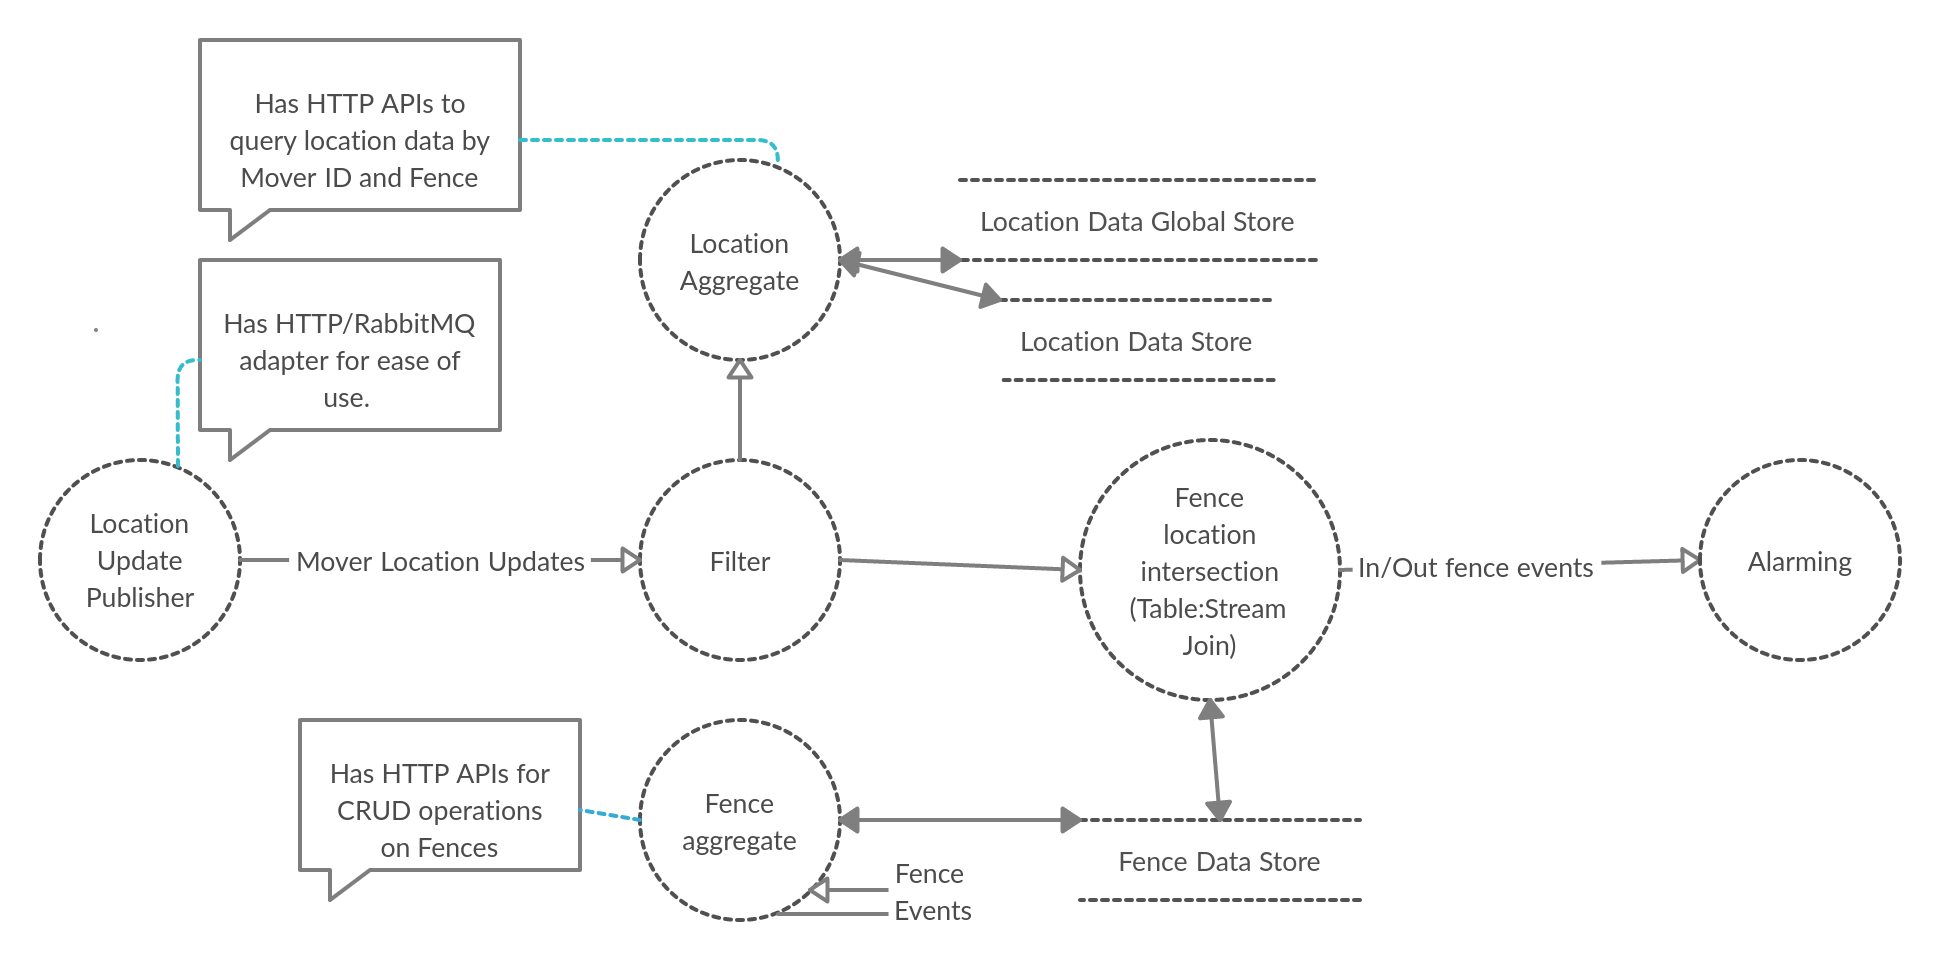
\includegraphics[scale=0.2]{images/logical-data-flow-diagram.png}

    \end{figure}

    \paragraph{location-update-publisher} plays the role of source in the FenceX stream processing pipe line.
    It has HTTP and RabbitMQ adaptors which is used by movers.
    Movers send messages or http requests in order report their latest location.
    Location-update-publisher turns each report into a event and publishes it into a kafka topic called \textbf{location-updates}.

    \paragraph{filter}, as the name suggests, is responsible for avoiding not desired location updates to find their way further down in the stream. Checks can be against null values or invalid latitude/longitude.

    \paragraph{location-aggregate} is responsible for keeping a view of latest location of each mover by subscribing to the stream of location updates coming out of filter. It has a local database of mover-locations which applies geospatial index on the data. As a result, the query by fence is becomes possible. So location-aggregate is responsible for answering queries both by mover id and fence (geospatial shape).

    \paragraph{fence-aggregate} is responsible to keep track of predefined fences (for real time intersection scenarios).
    It exposes HTTP APIs for CRUD operations.
    The fences are kept in an temporal KTable (kafka streams notion of table) and backed by a durable Kafka topic.
    In other words, each operation (CRUD) on each fence is initially a Kafka event which is later processed by fence-aggregate into a fence. The producer of those events is also fence-aggregate. In more technical terms, fence-aggregate is using event-sourcing architecture internally.

    \paragraph{fence-location-intersection} (join) has a view of predefined fences (managed by fence-aggregate) in shape of a key:value table.
    Key is id of mover for which the fence (value) is defined.
    fence-location-intersection is a join between that table and stream of location updates coming out of filter.
    Those location updates also has a key:value form. Key is the mover id and value is the reported location.
    And finally, the join operation is to check if the fence in table contains the location in the update.
    The result of this intersection will be events like mover X is (not) in the predefined fence.

    \paragraph{alarming} is responsible for responding to the events coming out of fence-location-intersection.
    Implementation of this operator is not withing boundaries of this thesis. So we won't describe its details.

    \subsection{Push and Poll legs}
    As described previously, FenceX provides two styles of geofencing, On demand and real time.

    Sending HTTP queries with a geospatial fence (query by fence) to FenceX is of on demand nature.
    Which means when ever a client demands a geofencing operation, they send a http query. In this style, fences are very dynamic.
    The fence will be checked against the whole data base of mover locations.
    \textbf{location-aggregate} is responsible for this style of fencing.
    Since sending query to a system is like polling data out of it, the parts of FenceX making this possible are considered poll leg.
    So \textbf{location-aggregate} is poll leg of FenceX.

    Calculating fence-point intersection for every location report, on the other hand, is of real time nature.
    For each new location report, system pushes a intersection calculation result.
    \textbf{fence-location-intersection and fence-aggregate} carry the burden of real time fencing and they are the push leg of FenceX.
    In this style the defined fences are more static and don't change frequently over time.

    From now on, we will use the notions of push and poll leg frequently specially in the evaluation phase, Each of these legs have their own characteristics and require individual attention.


    \section{Physical data flow graph}


    \begin{figure}[ht]
        \caption{Physical data flow graph of FenceX}
        \label{fig:physical-dfg}
        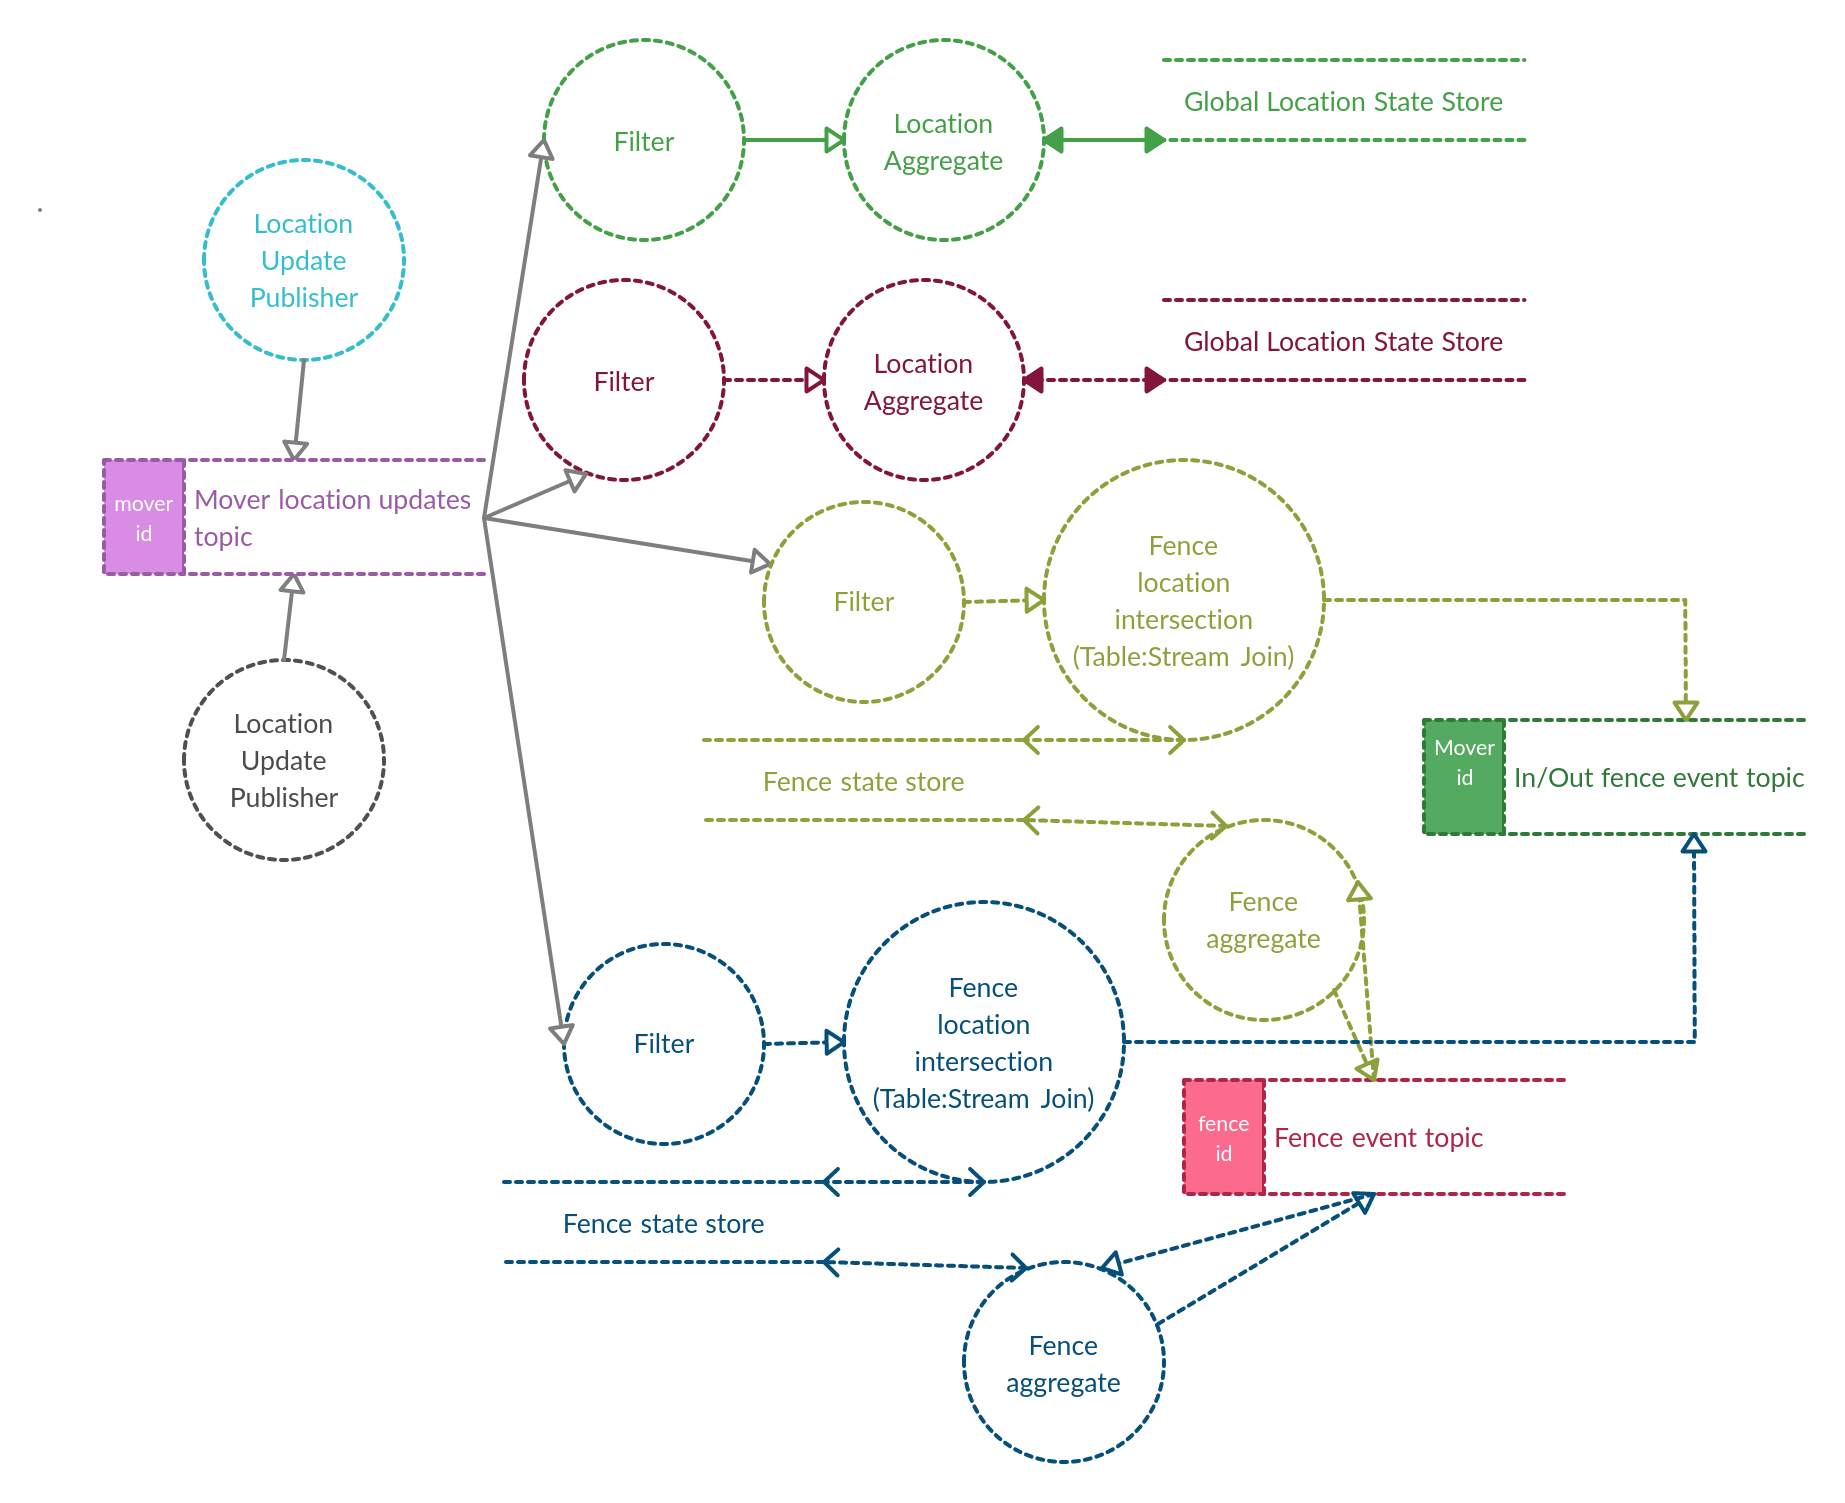
\includegraphics[scale=0.2]{images/physical-data-flow-diagram.png}

    \end{figure}

    Figure \ref{fig:physical-dfg} is a physical data flow graph, illustrating how possibly FenceX components can be deployed as instances of microservices containing stream processing pipe line tasks. Each group of tasks that has similar color, are one unit of deployment, an instance of a microservice.

    The combination of tasks below will be deployed as one microservice:
    \begin{itemize}
        \item{location-update-publisher} alone makes a microservice called \textbf{location-update-publisher}.
        \item{filter and location-aggregate} together make a microservice called \textbf{location-aggregate}. This the poll leg of FenceX.
        \item{filter, fence-aggregate and fence-location-intersection} together make a microservice called \textbf{realtime-fencing}. This the push leg of FenceX.
    \end{itemize}

    You can see that each microservice exists two times in \ref{fig:physical-dfg} differed by color. It means FenseX deploys more than one instance of each microservice for scalability and resiliency purposes.
    Such characteristics will be discussed in details later.

    Below are the facts common about all FenceX microservices:
    \begin{itemize}
        \item They are implemented using Java 15.
        \item They are implemented with extensive help from Spring family frameworks and libraries like Spring boot, Spring data, Spring webflux, Spring cloud and many more.
        \item They are packaged as layered docker images so the deployment artifacts of FenceX are docker images.
        \item So far all of them expose some HTTP APIs implemented using Spring webflux on top of project reactor. As a result they are reactive applications which means they process HTTP requests in a asynchronous and non blocking manner.
        \item All of them expose a HTTP API for fetching metrics about their resource usage, JVM status, geofencing operations and ... .
        \item After successful deployment, they will be registered into a service discovery tool called Consul.
    \end{itemize}

    \subsection{Inter microservices communication}
    At the moment there is no need for HTTP communication between FenceX microservices.
    However, they can find each other's IP by querying Consul on the fly.

    The communication style of microservices in FenceX is asynchronous and event driven.
    Which means there are Kakfa topics available for publishing events and subscribing to them.
    This topics are partitioned so each instance of the microservice will subscribe to a sub set of partitions.
    This is a load sharing strategy which helps with scalability.
    \ref{fig:physical-dfg} illustrates involved (Kafka) topics in the pipeline in addition to the state stores (database)
    attached to/used by each task.
    Fundamentally each of those state stores are backed by a topic (changelog).


    \section{Microservices internal design and implentation}
    Apart from common fact stated preciously, FenceX microservices can be described in a more detailed way as following:

    \subsection{Location-update-publisher}
    Location-update-publisher is a simple Kafka publisher.
    A source in the stream processing pipeline.
    It can be exposed to outside world using both RabbitMQ and HTTP adapters.
    The adapters receive location reports.
    Reports will be mapped to the event schema that other microservices
    understand and finally the event will be published into a topic called \textbf{location-updates}.
    This is a stateless service, so it can be scaled out very easy.
    Since the functionality of this service is simple, each instance doesn't need to be rich in resources.

    \subsection{location-aggregate}
    Location-aggregate is a Kafka Streams application.
    It's internal stream starts with subscribing to\textbf{location-updates}, continues with a filter and finally
    aggregated into a Global KTable which is backed by an in-memory H2 database.
    Which means once a location report received by location-aggregate, it will be first checked for validity and then
    saved into an in-memory co-located database.
    The save is an update operation most of the time.
    Updating the latest captured location for a mover.
    H2 provides geospatial indexing.
    Upon each update, the index will be updated as well, so the database will become ready for being queries against a
    fence.
    By database, we mean a single big table.

    \subsubsection{co-located database}
    Usually in information systems, databases have their own cluster and deployed on machines other than the one on
    which applications are deployed.
    This is done in order to abstract away availability and scalability challenges of data(base) from developers.
    The disadvantage is that accessing such a database can only happen over network which is an IO operation with
    relatively high latency.
    Since we aimed for high throughput (low latency) geofencing in FenceX, we decided to use a databases process
    deployed tightly together with location-aggregate.
    The life cycle of this database is managed by location-aggregate.
    In fact, it's a library within the application.
    In summary, we used an embedded database.
    The direct result is that the network call for accessing this database is only within range of localhost, so the
    latency is minimum.

    \subsubsection{In memory database}
    Usually database systems are configured to use disk as storage which allows them to grow very big.
    The downside with this approach is the IO intensiveness of interacting with disk which means latency.
    Although very high throughput SSD hard drives exists, not only their price tag is high but also they are still
    not as fast as memory.
    Our goal being minimizing IO latency, the H2 database not only is configured to use memory as storage but also
    using it in an asynchronous non-blocking manner (nioMemFS).
    Which means H2 will act as if a file system exists on the memory and will access it using Java NIO technology.

    \subsubsection{Inconsistency}
    Using database systems maintaining their own dedicated cluster, means no need for being worry about the
    possible inconsistency problems.
    The nodes in the cluster need to be consistent after all, even if only they act as cold idle replicas.
    Co-located in memory databases, on the other hand, usually doesn't have any consideration for replication and/or
    consistency.
    Since we want to scale out poll leg of FenceX, facing inconsistency issues is inevitable.
    So we need a way to make each instances of location-aggregate (all of the H2 instances) have same data, same
    image of the world.
    H2 provides an out-of-the-box solution for keeping its instances consistent, even when configured to be embedded
    and in memory.
    However, after some trial and error we did not find it reliable.
    So it is up to us to keep the instances of location-aggregate consistent.
    Kafka Streams Global KTables are state stores that have same data regardless of instance.
    They are equivalent to kafka subscribers each having a different group name;
    which means they get events from all partitions.
    Normal KTables only keep a subset of world image which corresponds to the partitions they listen to.

    So if we put the H2 database underneath a Global KTable, Kafka Streams out of box keeps the H2 instances
    consistent.
    \textbf{Eventually consistent} However!
    Eventually consistent means the consistency of data among instances of location-aggregate is not of ACID nature.
    Once a location update is published, the time taking for each instance to capture the location update and change
    its state accordingly, varies from an instance to another.
    This time is a factor of, for example, current load of each instance.

    Each Kafka Streams state store is backed by a topic called change log.
    This topic is durable and is saved on disk by kafka.
    Each Kafka Streams application attached on such a store, subscribe to that topic once it's up and running and
    populate it's KTables.
    That topic contains all changes that has happened to the state of application, the data in the KTable.
    So in case something happens to one of the instances (or all of them for that matter), after a restart or bringing
    a new fresh instance up, the instance recover/creates it own images of the world just by subscribing to change
    log topic.
    The subscription can be from last seen offset or from offset zero, depending on the state of underlying store.
    Sometimes the stores are back by a database using file system as storage.

    So finally we resolved the mystery of inconsistency in FenceX. Also, we covered some aspects of the work which
    makes FenceX high throughput.

    \subsection{realtime-fencing}
    Realtime-fencing is a Kafka Streams application responsible for keeping track of fences, receiving location updates
    and joining them.
    The join operation is fence-point intersection.
    It has two internal streams.
    One for processing location updates, and the other is for aggregating fences.

    \subsubsection{event-sourcing}
    One of the internal streams starts with subscribing to \textbf{fence\_event\_log} topic.
    The publisher to this topic is realtime-fencing itself.
    It exposes two HTTP APIs CRUD operations on fences (only create is implemented for now).
    When create fence API, for instance, is called, apart from possible initial validations, the
    only thing that happens is publishing an (kafka) event to \textbf{fence\_event\_log} topic.
    \textbf{fenceCreatedEvent} in this case.
    No fence is created yet or saved anywhere in the system, however that's how an event-sourcing based application
    works.
    The stream that starts with subscribing to \textbf{fence\_event\_log} topic, receives those events and aggregates
    them into a Kafka Streams KTable.
    A key:value table in which key is the ID of mover for whom the fence is defined;
    value is the WKT string describing the geospatial shape of the fence.
    Any operation on the fences should first be published as an event and later caputured by realtime-fencing up and
    running instances.
    The event will be processed, and a suitable change will happen on the data in the related state store.
    This approach (event-sourcing) is one of special styles of event driven architectures which feels very natural
    when implemented using Kafka Streams.
    Using this architecture leads to a eventual consistency which is usually the case with all event based systems.
    The benefit is the huge potential for scalability.
    Also, the source of truth in such systems is the event\_log topic rather then the database (state store).
    Whatever happens to the whole application, the state can be easily recovered by bringing a new instance of
    application up and making it subscribe to event\_log topic from offset zero.
    Or in case of a bug in business logic that resulted in a wrong state, a correct state can be rebuilt after fixing
    the bug.
    These benefits come from the fact that the only durable data in this architecture is immutable facts, the
    events that has happened.
    It's worthy to mention that the event\_log topic can be used as an activity log for monitoring and debugging purposes.

    In realtime-fencing the KTable keeping the fences is backed by a change log style topic similar to what we
    described about location-aggregate.
    The difference here however is that the KTable keeping fences is not global.
    So each instance of realtime-fencing has a subset of defined fences corresponding to the partitions of
    kafka topic listening to.
    Since load balancers does not know what instances is responsible for what fences at any given point in time, in
    order to query this KTable, a select all query for example, each instance that receives the query, will gather
    data from other instances.
    Such data gathering should be party implemented by us using some related features of Kafka Streams.
    In case queries more complex than select one or select all were required, this approach would not work.
    Mainly because the KTable is only a simple key:value table.

    So far we described one the internal streams of realtime-fencing, the one related to aggregating fences.

    \subsubsection{Join stream}
    The other internal stream of realtime-fencing starts with subscribing to \textbf{location-updates}, continues with a
    filter and finally a join operation.
    A join between this stream of location updates and the table of fences.
    The stream is a key:value stream.
    Key is the mover ID for whom the value, location report, is published.
    A join between this stream and the fence KTable means whenever a new location update is received for a mover,
    the fence defined for that mover (if exists) will be fetched.
    Now a function can be called with the these inputs: ID of mover, the defined fence and the newly received location update.
    In our case implementation of the function is calculating if the new location is within the defined fence, A
    geospatial point-shape intersection.
    Which we call point-fence intersection.
    Output of function should be a Key:Value pair with the mover ID being the key and the value is result of
    intersection.
    So after the join we end up with a stream of moverId:intersection-status updates.
    At the moment we have not continued the stream but ideally the status should be published into another kafka
    topic so that other operation down the stream processing pipeline can use it, like alarming.


    \section{Non functional characteristics}
    In this section we describe how different non-functional requirements of system has been achieved based on the
    design and architectural decisions.

    \subsection{Availability}
    Availability has many aspects in software development specifically when it comes to distributed systems.
    The main practice to achieve high availability is to scale out meaning deploying more than one instance of the
    application, application subcomponents for that matter.
    In case of microservices, more than one instance of each microservice should be deployed.
    In the same way deploying more than one task of each operation makes sense in stream processing realm.
    The benefits of scaling out in terms of availability are as following:
    \begin{itemize}
        \item[Operational availability] If a sub set of deployed services stop responding for any reason, the rest of
        up and running instances
        can take over the work.
        \item[Data availability] Data can be replicated over different instances of services so if something goes
        wrong with one of the instances, the data will not get compromised.
        The process of data can even be continued without any special change being noticed in the overall behaviour of
        system.
        \item[Availability under varrying load] Will be explained as scalability in the next section
    \end{itemize}

    In FenceX it's easily possible to deploy as many instances of microservice as required by non-functional boundaries
    of corresponding users and use cases.
    We use a container orchestration tool called Nomad for managing deployment of FenceX microservices.
    Which allows for a joyful experience of managing containers.
    While being a full fledged production level container orchestration tool, It's not as complicated as Kubernetes.

    \subsubsection{back pressure}
    ???

    \subsubsection{rebalancing}

    \subsection{Scalability}
    A software system being scalable in simple terms means that system can handle different sizes and frequencies of
    input load successfully.
    There are different elements in a software system that can grow:
    \begin{itemize}
        \item Data size in data bases
        \item API call (incoming HTTP requests for example)
        \item Input rate in stream processing systems (Rate at which events arrive)
        \item Number of parallel inter dependent operations
        \item Number of parallel independent operations
        \item Number of active threads in the thread based systems
        \item Queue size (number of events in kafka topic for example)
        \item Stack size
        \item Number of users using the system at the same time
        \item Number of system subcomponents (number of microservices or number of stream processing operations)
        \item Number of people can work on development the system at the same time (organizational scalability)
    \end{itemize}
    A scalable software system keeps responding/processing successfully with reasonable throughput and latency even if
    any (or all) of the factors mentioned above grow hugely in size or in rate.
    The growth can happen step by step over a window of time or like a sudden sock in a moment.

    \subsubsection{Data scalability}
    In FenceX data scalability is limited by the number of rows that an H2 in memory table can keep. Which is ??.
    This can be limited because each H2 in memory table in FenceX is below a global KTable which means it has the whole
    image of world.
    Otherwise the other stateful operation is fence-aggregation which is highly scalable in terms of data due to the
    fact that data in that state store, is partitioned over available instances of realtime-fencing.
    So if defined fence sizes grow, horizontally scaling realtime-fencing will just deal with it.

    \subsubsection{incoming HTTP requests}
    All HTTP APIs in FenceX are implemented using reactive stack (instead of thread based servlet stack) using Spring
    webflux library.
    Reactive in this context means asynchronous non-blocking IO which allows each instance to process much more HTTP
    requests providing having same resources.
    In simple terms no CPU cycles will be wasted for/while WAITING for IO results.

    Also, deploying more than one instance of each microservice allows for load distribution.
    A load balancing solution (client side load balancing in case of FenceX) distributes the HTTP calls over up and
    running instances of target microservice.
    So more requests can be responded at the same time.
    This is called scaling out which is opposite to scale up.
    When scaling up, we increase the resources available to each component, to each instance.
    Scaling up (scaling vertically) is usually expensive and does not provide other types of scalability
    (organizational scalability for example).

    \subsubsection{stream processing systems input rate}
    In event driven systems specifically stream processing ones, the input is incoming events and messages waiting to
    be processed.
    Location reports in case of FenceX.
    For FenceX to be able to handle high rates of input, the events are published into Kafka topics.
    Kafka topics are partitioned.
    Each task (microservice instance) once is up, healthy and ready for processing, subscribe to a subset of those
    partitions.
    Which means the event processing load is distributed among available tasks.
    This is called \textbf{data parallelism} in stream processing.
    When same tasks process different data.
    Appying this, which is basically scaling out, allows for dealing with high rates of input.
    Just by deploying more instances of microservices, we end up having more capacity for processing incoming events.
    It is by the way very important to have more partitions than number of deployed instances.
    Otherwise, we will end up with idle tasks.

    \subsubsection{Design and organizational complexity}
    Over time as system evolves and provides more functionality, keeping all the codes in one service brings various
    non-technical problems.
    In short, we will end up with one big service which is very hard to maintain, deploy, debug, build, reason about
    and most importantly change.
    In such service everything is couple together due to high reliance on code reuse.
    The alternative is to break down this monolith into different microservices each of them responsible for doing
    mainly one thing.
    They will have their own database, build and deployment process and ... .
    These microservices ideally share nothing and communicate ONLY using messages (reactive).
    Such de coupled microservices can be introduced over time to the whole system when ever new requirements requires so.
    This way development and design of new features is independent of others;
    so the best fitting internal architecture, language, database, code style and ... can be selected for that specific
    service.

    Such an independence also allows multiple people, multiple teams for that matter, to work at the same on the same
    overall system.
    There is a practical limit on how many people can work at the same time on the same code base as an example.
    When system code is distributed over different code bases, a lot of people can work at the same time on the
    system and deliver value.

    \subsubsection{other scalability aspects}
    ?????

    \subsection{Throughput}
    For FenceX throughput of two types of operations matter the most.
    Throughput of HTTP requests for querying the database of locations against a fence (poll leg throughput).
    And, throughput of fence-point intersections (push leg throughput).
    Throughput is usually closely related to scalability since high throughput is achievable only under high input
    load.

    \subsubsection{Poll leg throughput}
    Is the number of queries (by fence) that FenceX can respond to successfully in a unit of time (seconds).
    This throughput is a factor of number of queries one can send to FenceX which is the input rate in the poll leg
    context.
    Another effective factor is the latency of each query.
    This latency depends on the amount of IO involved, geospatial index algorithm, network access latency, CPU speed
    and number of parallel queries.
    In FenecX we minimized the network latency and IO latency by using an embedded co-located in-memory database.
    Also using reactive programming for implementing HTTP APIs, removes the latency that waiting for blocking IO
    operations imposes.

    Also, using microservices architecture and scaling out the poll leg instances leads to more capacity for responding
    to simultaneous queries.

    We calculate the poll leg throughput by increasing a counter everytime FenceX respond to a query successfully.
    This counter is a metric gathered every now and again by a time series database called Prometheus.

    \subsubsection{Push leg throughput}
    Is the number of fence-point intersections that FenceX can calculate in a unit of time (seconds).
    This throughput depends on the input rate (rate of incoming location updates) and how many instances of push leg
    are up and running.
    By scaling the realtime-fencing microservice out, we allow for parallel intersections to happen (data parallelism).
    Which means FenceX can calculate more intersections per unit of time.
    The trigger for each intersection operation is a location update which is received as a kafka event coming through
    kafka topic partitions.
    So theoretically number of partitions in the kafka topic is also a factor.

    We calculate the push leg throughput by increasing a counter everytime FenceX calculates a fence-point intersection.
    This counter is a metric gathered every now and again by a time series database called Prometheus.


    \section{Underlying Ideas and sciense}
    In this section we cover the architectural and scientific ideas which play fundamental roles in this thesis.
    We cover them only to the extent that context of this thesis allows.

    \subsection{Stream processing}

    \subsection{Geofencing}

    \subsubsection{WKT}

    \subsection{Microservices}


    \chapter{Evaluation}
    In this chapter we explain the process and results of evaluating FenceX.
    This process consist of many experiments with different setup and goals.
    Each experiment had a preparation phase, execution, observation and finally comparison.


    \section{Deployment}
    The deployment configuration for FenceX microservices in production depends on the exact needs of business.
    It is also always limited to the hardware resources available, like any other software.
    During evaluation of FenceX for this thesis we had access to 4 virtual machines with the following resources
    available to them.
    \begin{center}
        \begin{tabular}{ c c c c}
            Server  & CPU CORES & RAM(GB) & Main responsibility \\
            server1 & 8         & 16      & Master keeper       \\
            server2 & 4         & 8       & Nomad worker node   \\
            server3 & 4         & 8       & Nomad worker node   \\
            server4 & 4         & 16      & Benchmarking        \\
        \end{tabular}
    \end{center}


    Figure \ref{fig:infrastructure} illustrates how FenceX deployment looks from infrastructure point of view in a
    possible evaluation scenario.
    The only difference compared to other evaluation scenarios is the number of deployed instances of FenceX
    microservices like realtime-fencing.

    \begin{figure}[ht]
        \caption{FenceX infrastructure setup for evaluation}
        \label{fig:infrastructure}
        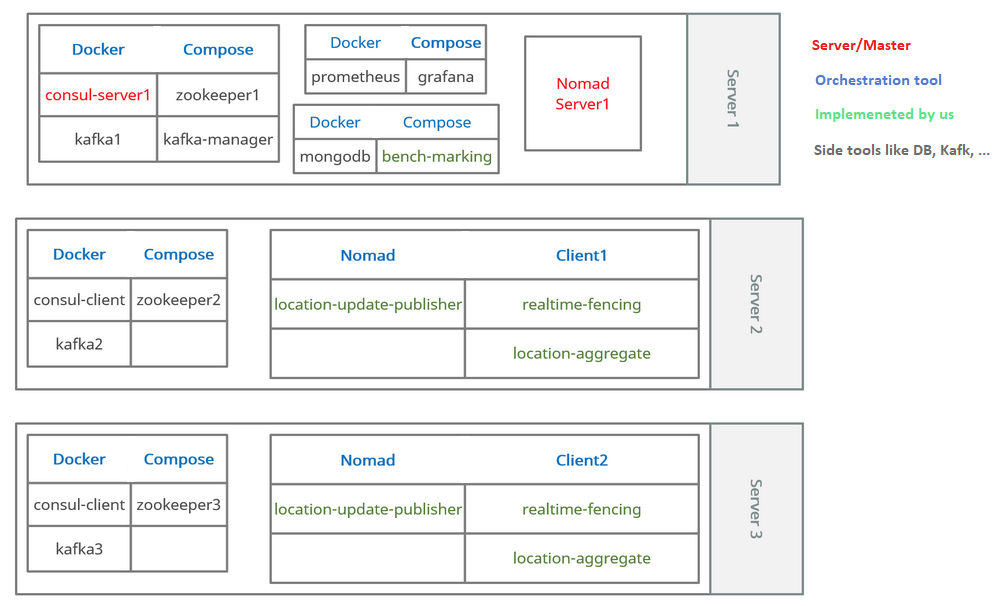
\includegraphics[scale=0.6]{images/Infrsutracture.png}
    \end{figure}

    \ref{fig:infrastructure} does not include server4 since that server only run an instance of benchmarking app
    which is not part of the FenceX solution package.
    Nevertheless, we have deployed another instance of bench-marking into server1 getting high throughput out of
    bench-marking applications is a very expensive in terms of resources.

    It is also important to note that FenceX had 4 major Kafka topics.
    \textit{fence\_event\_log, location-aggregate-mover-in-memory-state-store-changelog, mover-position-updates,
        realtime-fencing-fence-state-store-changelog}
    All of these topics were configred to have 3 replicas and 12 partitions.
    These numbers are selected corresponding to availalbe resources to the overal system.
    The process of selecting them correctly is out of the countext of this thesis.
    The important factor however is to have a high enough replication factor to achieve availability (3 at least) and
    high enough number of partitions to avoid idle subscribers.

    \paragraph{}
    After preparing the infrastructure, Nomad calculated the whole available resources to the application that will
    be deployed into worker nodes as 16670 MHz of CPU cycles and 16 GB of memrory. ??? I'm not sure it's CPU power
    per core or in totall???

    \subsection{Bench-marking app}
    Before diving into the test cases, it worth the effort to explain how bench-marking app works and what options it
    provides.

    Generally speaking it is a microservice similar to other services in FenceX.
    It registers itself into Consul and has HTTP APIs.
    It is based on spring-webflux reactive stack in order to handle IO better.
    The role of bench-marking is to imitate the behaviour of real world mover location report publishers,
    smartwatches or car gps modules for example.

    bench-marking has a dataset of real taxi trips ??thanks to Cabonline generousness??.
    Each trip has an anonymized ID, a set of location reports (points), a geospatial circle (fence) drawn around one of
    those
    points.
    The points are in form of coordinates (latitude, longitude) and the fences are WKT strings.
    Eah trip has an average of 17 points and in total around 500 trips are in the database.

    \paragraph{}
    bench-marking can send HTTP requests to realtime-fencing and define fences for movers.
    For simplicity mover ID will the trip ID.

    \paragraph{}
    bench-marking can send HTTP requests to locatin-update-publisher and report coordinates for each trip.
    The result in FenceX will be stream of location updates published into the pipeline.

    \paragraph{}
    bench-marking can send HTTP requests to location-aggregate and query its location database against the fence
    defined for each trip.

    bench-marking can do operations mentioned above for all the trips repeatedly very fast in order to push a
    stressful load of inputs into the FenceX pipeline.
    It can also keep the size of load low while keeping it ongoing (non-stop) over time.

    It appeared that producing stressful loads of HTTP request or ongoing flows of them is a very expensive operation
    in terms of memory usage and CPU usage to some extent.
    Mostly during our evaluations the bottleneck to throughput was our input rate.


    \section{Pure throughput}
    In this section we go over the experiments we have conducted in order to not only stress test FenceX but also
    calculate the peak throughput based on overall available resources.
    Throughput is a direct factor of input rate both for on demand poll style operations and realtime push style ones.
    In on demand style, the input rate is the number of HTTP reuqests per second that system receives.
    For realtime operations, the input rate will be number of location reports arrived at system per second.
    As mentioned previously, for each setup, exists a threshold for input rate above which throughput won't go any
    higher by increasing input.

    \paragraph{}
    In order to calculate the throughput in each experiment, we use a combination of tools, Prometheus and Grafana.
    Prometheus is a time series database that polls different types of metrics out of each of our FenceX
    microservices on a frequent basis.
    Grafana is a visualization tool that reads metric data from Prometheus and illustrates it into a veriety of graphs.
    The metrics can be general like CPU usage or number of JVM threads.
    They can also be custom to each application like number of fence-point intersection calculations.
    Using this setup, we created realtime graphs that shows pull and push throughput of FenceX in addition to other
    information like push and poll input rate.
    As a result we do not need to calculate the throughput after each experiment.
    We can just have a look at corresponding graphs during execution of test scenario in order to see the realtime
    value of throughput and input rate.

    \subsection{Push leg}
    The process of push throughput experiments are as following:
    \begin{itemize}
        \item[1-] Define fences for movers using all the trips in the bench-marking application database.
        \item[2-] send a shocking stream of location reports into the FenceX.
        \item[3-] Check the throughput.
        \item[4-] Repeat the experiment after changing the deployment configuration. (Maybe add more instances or add
        more CPU) until finding peak throughput and/or a possible upper bound on throughput.
    \end{itemize}

    \subsubsection{Experiment 1}

    \paragraph{Deployment view}
    \begin{center}
        \begin{tabular}{ c c c c }
            Application               & number of instances & CPU(MHz) & RAM(MB) \\
            location-update-publisher & 4                   & 500      & 500     \\
            location-aggregate        & 3                   & 2000     & 2500    \\
            realtime-fencing          & 4                   & 700      & 800     \\
        \end{tabular}
    \end{center}

    \paragraph{Results}
    \begin{figure}[ht]
        \caption{FenceX push throughput ex1-1}
        \label{fig:ex1-1}
        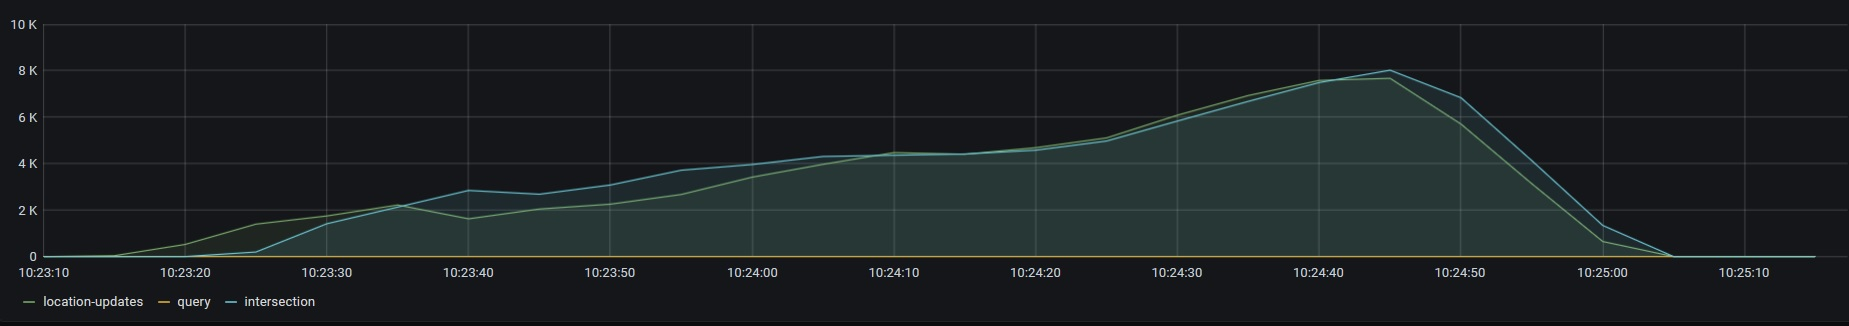
\includegraphics[scale=0.4]{images/evaluation/ex1-benchmarking(15,6).png}
    \end{figure}

    \begin{figure}[ht]
        \caption{FenceX push throughput ex1-2}
        \label{fig:ex1-2}
        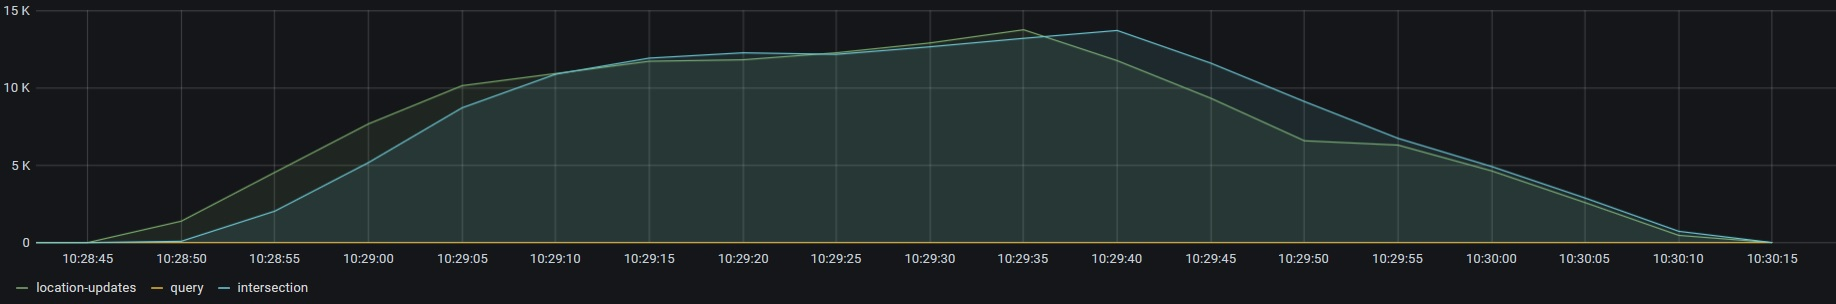
\includegraphics[scale=0.4]{images/evaluation/ex1-benchmarking(19,7).png}
    \end{figure}

    \begin{figure}[ht]
        \caption{FenceX push throughput ex1-3}
        \label{fig:ex1-3}
        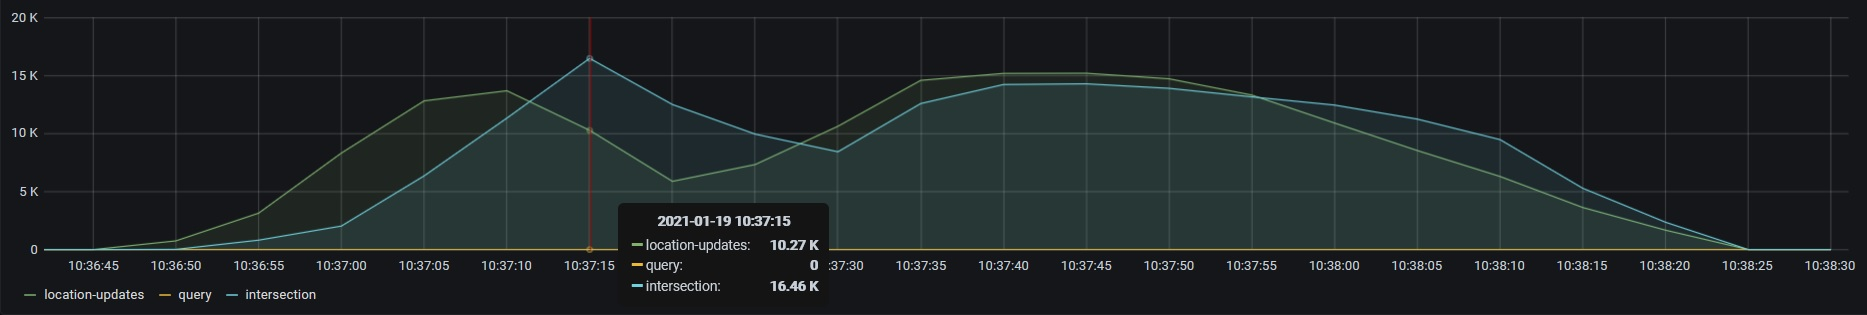
\includegraphics[scale=0.4]{images/evaluation/ex1-benchmarking(22,9).png}
    \end{figure}

    \begin{figure}[ht]
        \caption{FenceX push throughput ex1-4}
        \label{fig:ex1-4}
        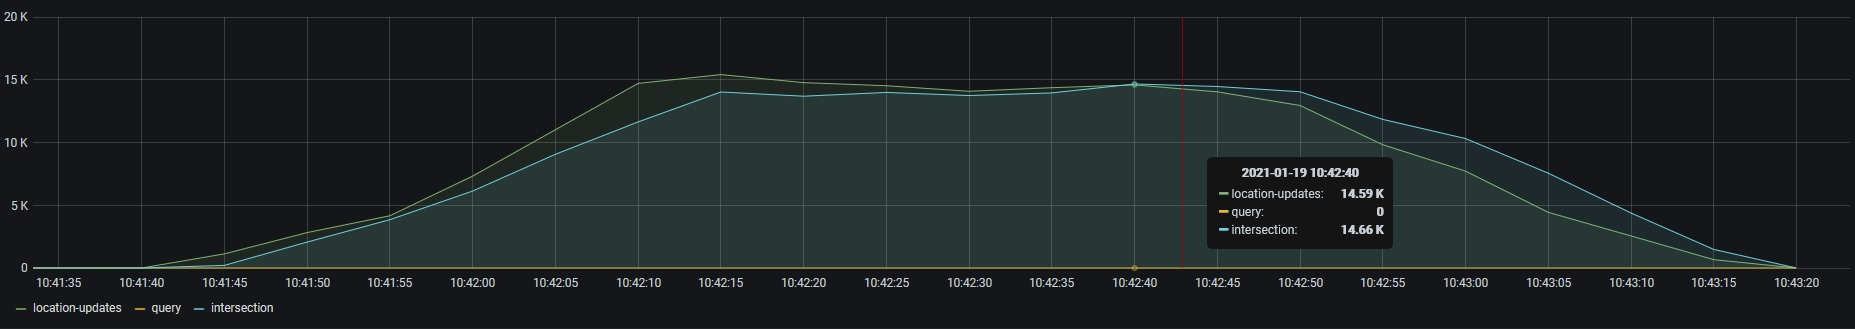
\includegraphics[scale=0.4]{images/evaluation/ex1-benchmarking(23,10).png}
    \end{figure}

    The figures \ref{fig:ex1-1}, \ref{fig:ex1-2}, \ref{fig:ex1-3} and \ref{fig:ex1-4} illustrate input rate
    (location-updates per second) with green line and push throughput (number of fence-point intersection
    calculations per second) with the blue line.
    These figures show that when we tried different input rates (ranging from 8k/s to 15k/s), the throughput was
    following the change patterns in input rate.
    Also, throughput were mainly always as high as input rate.
    The highest input rate we managed to produce during these experiments was around 15K location updates per second
    and FenceX just managed to handle it very well with the given deployment setup.

    \subsubsection{Experiment 2}

    \paragraph{Deployment view}
    \begin{center}
        \begin{tabular}{ c c c c }
            Application               & number of instances & CPU(MHz) & RAM(MB) \\
            location-update-publisher & 5                   & 400      & 700     \\
            location-aggregate        & 3                   & 2200     & 2600    \\
            realtime-fencing          & 5                   & 400      & 700     \\
        \end{tabular}
    \end{center}

    \paragraph{Results}
    \begin{figure}[ht]
        \caption{FenceX push throughput ex2}
        \label{fig:ex2}
        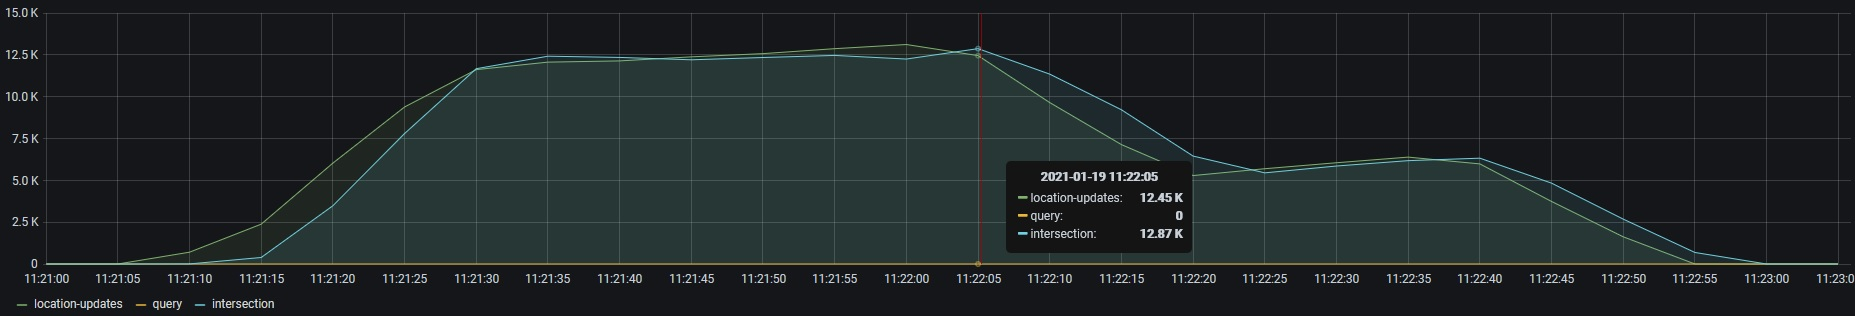
\includegraphics[scale=0.4]{images/evaluation/ex2-benchmarking(24,10).png}
    \end{figure}
    The figure \ref{fig:ex2} can be read in the same way as figures in experiment 1.

    So far the bottleneck is input rate which is limited by our physical resources available to bench-marking
    application.
    We can clearly see in the graphs that regardless of setup, push throughput (intersections/sec) follows pretty
    much the exact parent of changes in input rate (location updates/sec).
    So there is no point in continuing push throughput experiments with current available hardware power.

    \subsection{Poll leg}
    The process of poll throughput experiments are as following:
    \begin{itemize}
        \item[1-] Define fences for movers using all the trips in the bench-marking application database.
        \item[2-] Send a many location updates to FenceX.
        \item[2-] Send a shocking load queries (query by fence) to FenceX.
        \item[3-] Check the throughput.
        \item[4-] Repeat the experiment after changing the deployment configuration. (Maybe add more instances or add
        more MEMORY) until finding peak throughput and/or a possible upper bound on throughput.
    \end{itemize}

    \subsubsection{Experiment 3}

    \paragraph{Deployment view}
    \begin{center}
        \begin{tabular}{ c c c c }
            Application               & number of instances & CPU(MHz) & RAM(MB) \\
            location-update-publisher & 4                   & 500      & 500     \\
            location-aggregate        & 2                   & 2500     & 3200    \\
            realtime-fencing          & 4                   & 700      & 800     \\
        \end{tabular}
    \end{center}

    \paragraph{Results}
    \begin{figure}[ht]
        \caption{FenceX push throughput ex3}
        \label{fig:ex3}
        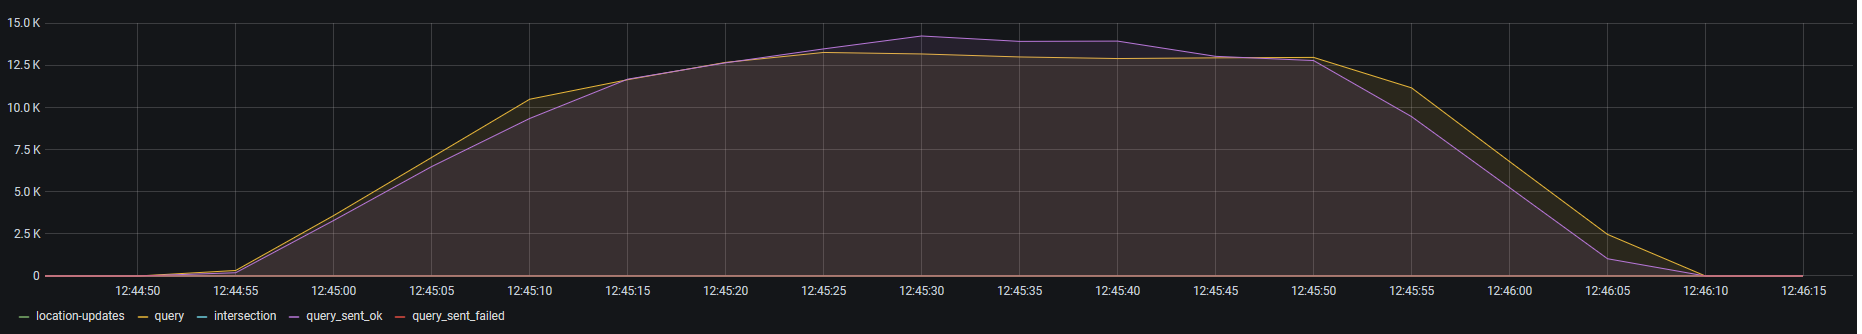
\includegraphics[scale=0.4]{images/evaluation/ex3-benchmarking(16,9).png}
    \end{figure}

    Figure \ref{fig:ex3} illustrates input rate (queries sent successfully per second) with purple line and poll
    throughput (number of queries answered without error) with the yellow line.

    \subsubsection{Experiment 4}

    \paragraph{Deployment view}
    \begin{center}
        \begin{tabular}{ c c c c }
            Application               & number of instances & CPU(MHz) & RAM(MB) \\
            location-update-publisher & 4                   & 500      & 500     \\
            location-aggregate        & 2                   & 2700     & 2700    \\
            realtime-fencing          & 4                   & 700      & 800     \\
        \end{tabular}
    \end{center}

    \paragraph{Results}
    \begin{figure}[ht]
        \caption{FenceX push throughput ex4-1}
        \label{fig:ex4-1}
        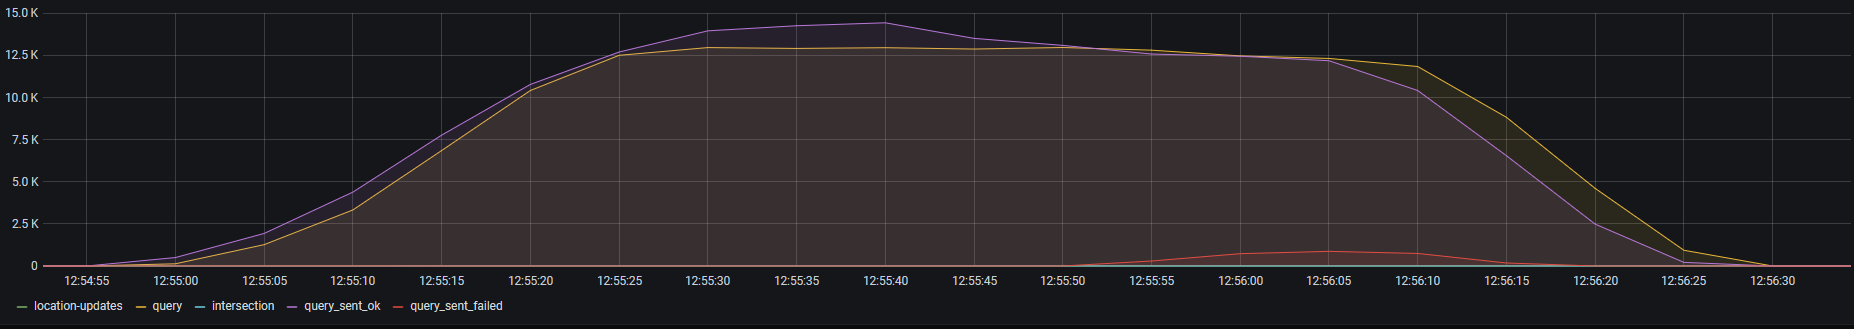
\includegraphics[scale=0.4]{images/evaluation/ex4-benchmarking(19,10).png}
    \end{figure}

    \paragraph{Results}
    \begin{figure}[ht]
        \caption{FenceX push throughput ex4-2}
        \label{fig:ex4-2}
        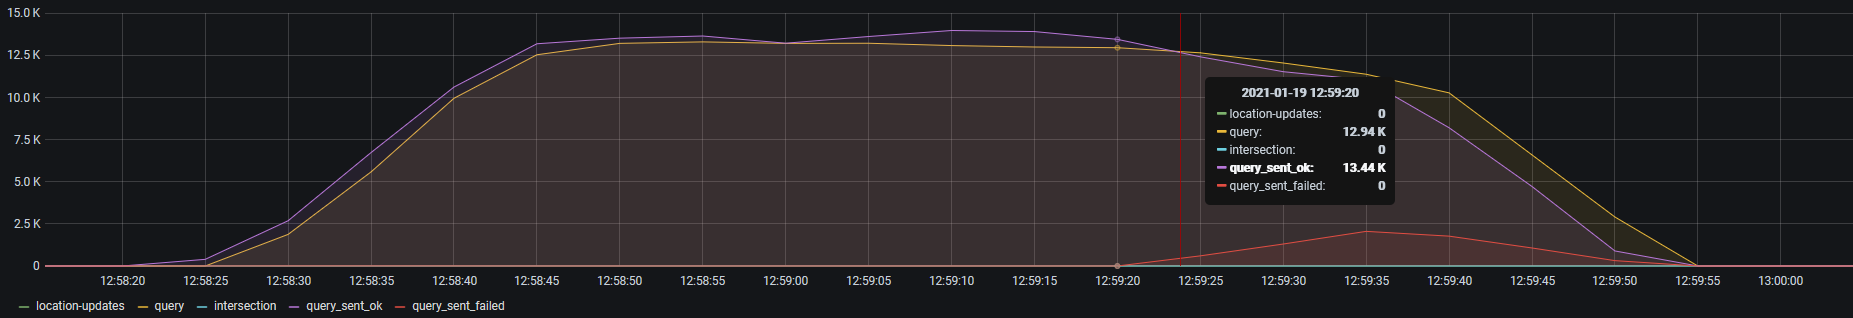
\includegraphics[scale=0.4]{images/evaluation/ex4-benchmarking(22,10).png}
    \end{figure}

    Both figure \ref{fig:ex4-1} and \ref{fig:ex4-2} can be read similarly to experiment 3 graphs.

    Experiments 3 and 4 show that we failed to increase the input rate as we progressed.
    So although the CPU usage on location-aggregate instances peaked to 100 percent during these experiments,
    again the bottleneck was input rate which is limited by our physical available resources.
    We can clearly see in the graphs that regardless of setup, poll throughput (queries/sec) follows pretty
    much the exact parent of changes in input rate (queries sent/sec).
    So there is no point in continuing poll throughput experiments with current available hardware.
    However, the highest input rate we managed to produce during these experiments was in the range of [12-13]K queries
    per second which FenceX just managed to handle very well.


    \section{Availability}
    In this section we cover the experiments we have conducted in order to test availability of FenceX.
    More precisely, we start an ongoing load or stream of input.
    Once throughput becomes stable, we restart one of the instances of involved microservices.
    The overall expectation is that during the restart, until the service becomes up and running again, the throughput
    goes down and afterward goes up again to the previous value.
    The main factor affecting the time takes until the service is up and running again is re-balancing.
    Kafka topics have consumer groups.
    Each member of a group, listens to a subset of partitions of that topic.
    This essentially results in data parallelism.
    A topic can have multiple groups listening to it which essentially is foundation of task parallelism.
    Re-balancing happens when one of the group members becomes unhealthy and stops subscribing to its assigned
    partitions.
    At this moment, other healthy group member should take over the dangling partitions.
    The processes of reassigning the dangling partitions to healthy subscribers is called re-balancing.
    The time a possibly successful re-balancing takes depends on the number of partitions and available
    healthy subscribers.
    So the time takes until throughput goes back to previous value is also not fixed.

    Please note that after a restart, there will be two re-balancings.
    One will be once the service under restart goes down and one once it come back up and running.
    If the remaining services after first re-balancing, had enough resources availalbe, the throughput won't change
    that much.
    Specially for lower incoming loads.

    \subsection{Push leg}
    The process experiments are as following:
    \begin{itemize}
        \item[1-] Define fences for movers using all the trips in the bench-marking application database.
        \item[2-] Start an ongoing stream of location report toward FenceX.
        \item[3-] Wait until throughput becomes stable.
        \item[4-] Restart on of the instances of realtime-fencing.
        \item[5-] Assert that throughput drops.
        \item[6-] Wait until successful re-balancing.
        \item[7-] Assert that throughput is back to previous value.
        \item[8-] Repeat the experiment with difference of restarting two instances instead of one.
    \end{itemize}

    \subsubsection{Experiment 5}

    \paragraph{Deployment view}
    \begin{center}
        \begin{tabular}{ c c c c }
            Application               & number of instances & CPU(MHz) & RAM(MB) \\
            location-update-publisher & 5                   & 400      & 700     \\
            location-aggregate        & 2                   & 2700     & 2700    \\
            realtime-fencing          & 6                   & 400      & 800     \\
        \end{tabular}
    \end{center}

    \paragraph{Results}
    \begin{figure}[ht]
        \caption{FenceX push leg availability ex5-1}
        \label{fig:ex5-1}
        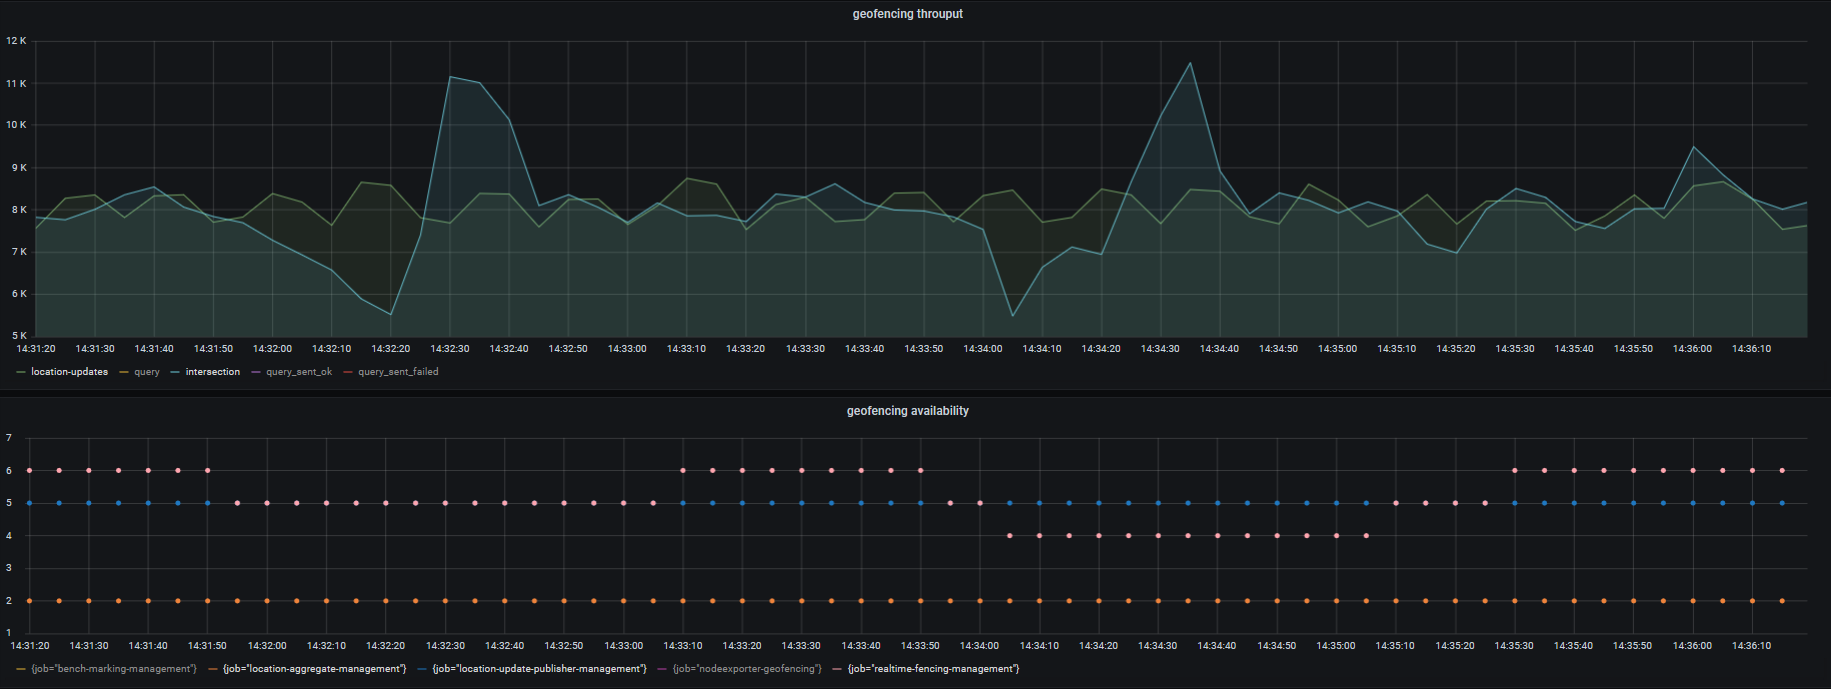
\includegraphics[scale=0.4]{images/evaluation/ex5-benchmarking-ongoing-2per7sec.png}
    \end{figure}

    \begin{figure}[ht]
        \caption{FenceX push leg availability ex5-2}
        \label{fig:ex5-2}
        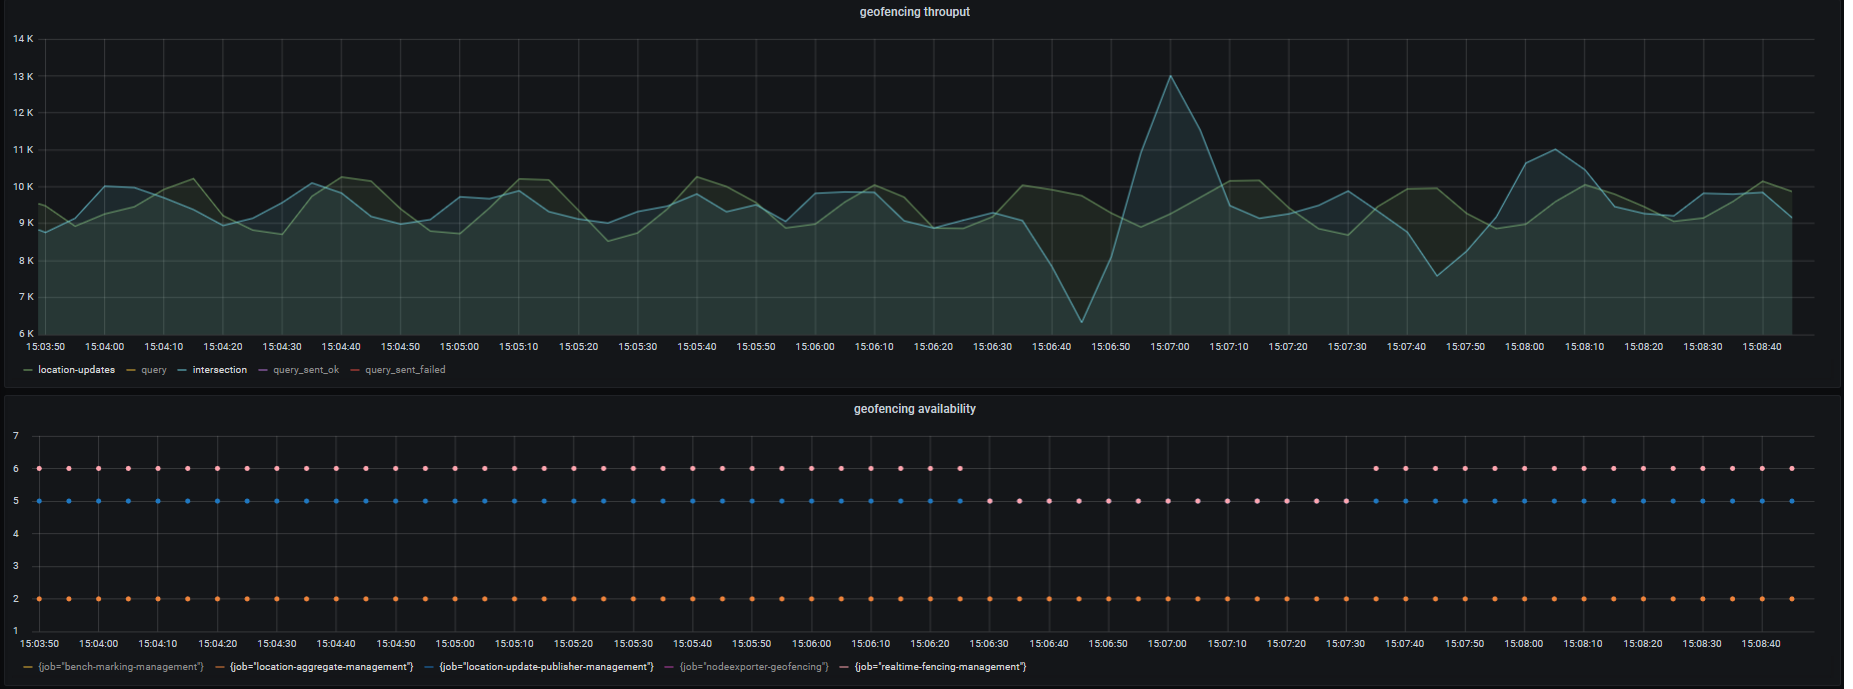
\includegraphics[scale=0.4]{images/evaluation/ex5-benchmarking-ongoing-2per6sec.png}
    \end{figure}

    In figures \ref{fig:ex5-1} and \ref{fig:ex5-2}, blue line represents the push throughput.
    Green line illustrates the ongoing input stream of location updates and pink point shows
    number of up and running realtime-fencing instances.
    As you can see in \ref{fig:ex5-1} and \ref{fig:ex5-2}, there are two points in the timeline at which number of
    realtime-fencing
    instances goes down (by 1 and 2) and later comes back to 6 again.
    During the time which takes for all 6 instances to be up and running again, throughput slightly drops and
    eventually recovers.
    Since we are using kafka topics as durable storage of location updates, the location updates which
    didn't get a chance to get processed, get it after re-balancing.
    As a result, we have even a higher throughput than input rate temporarily after re-balancing finishes.

    \subsection{Poll leg}
    The process experiments are as following:
    \begin{itemize}
        \item[1-] We defined fences and sent location updates for movers using all the trips in the bench-marking
        application database.
        \item[2-] Start an ongoing load of queries (query by fence) to FenceX.
        \item[3-] Wait until throughput becomes stable.
        \item[4-] Restart on of the instances of location-aggregate.
        \item[5-] Assert that throughput drops.
        \item[6-] Wait until successful re-balancing.
        \item[7-] Assert that throughput is back to previous value.
        \item[8-] Repeat the experiment with difference of restarting two instances instead of one.
    \end{itemize}

    \subsubsection{Experiment 7??}

    \paragraph{Deployment view}
    \begin{center}
        \begin{tabular}{ c c c c }
            Application               & number of instances & CPU(MHz) & RAM(MB) \\
            location-update-publisher & 0                   & 400      & 700     \\
            location-aggregate        & 4                   & 2700     & 2700    \\
            realtime-fencing          & 0                   & 400      & 800     \\
        \end{tabular}
    \end{center}

    \paragraph{Result}
    \begin{figure}[ht]
        \caption{FenceX poll leg availability ex7}
        \label{fig:ex7}
        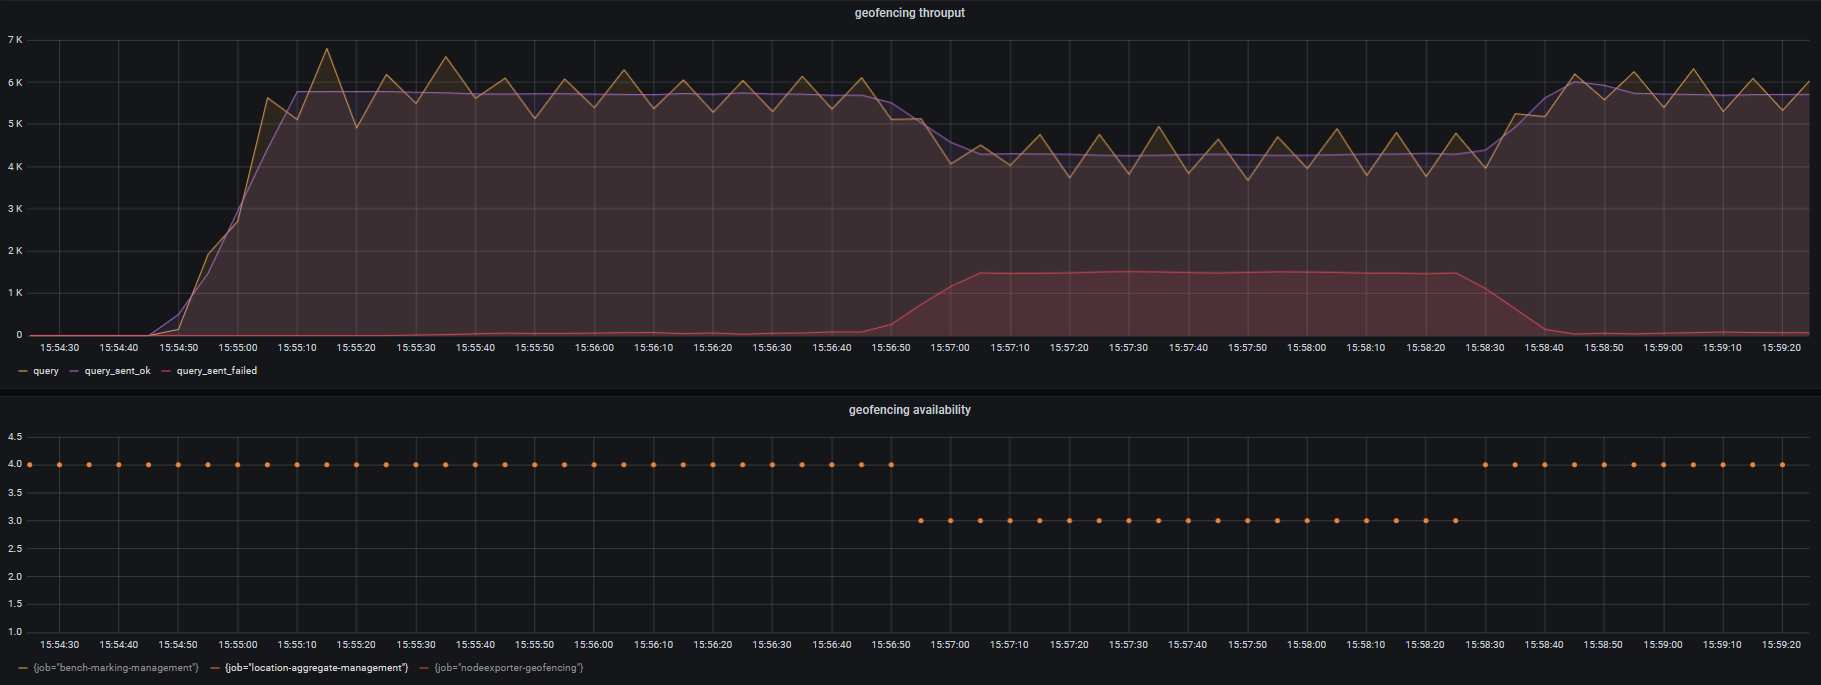
\includegraphics[scale=0.4]{images/evaluation/ex7-benchmarking-ongoing-2per10sec.png}
    \end{figure}

    In figure \ref{fig:ex7} the purple line is essentially the input rate (number of queries received by FenceX per
    second) and the yellow line shows the rate of queries answered successfully.
    Red line shows how many queires FenceX failed to respond.
    A failure to respond in this incoming load range means the service that was supposed to answer the query was not
    up and running (due to restart) at that moment.
    As you can see once restart and re-balancing finishes successfully, the throughput increases back to the previous
    value and error rate drop back to zero.
    Please note that re-balancing has no direct affect on queries by fence.
    However, health of each Kafka or Kafka Stream application is dependent to a successful re-balancing.


    \section{Strong scalability}
    If a software has strong scalability properties means providing same load, the more you scale it out, the better
    it performances.
    For a given circumstance, there might be a point after which scaling out more won't affect the performance anymore.
    The load can be data set size, table size, incoming http query rate and ... .
    Performance is also case and context dependent.
    It can be query latency, throughput and ... .
    In stream processing systems like the load is the rate of input, rate of incoming events, the rate at
    which source produces input in to the piple line.
    In FenceX, for poll leg, similar to previous experiments, load is rate of incoming HTTP requests for queries by
    fence.
    And, for push leg is the rate at which location reports arrive.

    Performance in case of our experiments for FenceX specifically, is throughput of push leg and poll leg.

    \subsection{Push leg}
    The process of strong scalability experiments are as following:
    \begin{itemize}
        \item[1-] Define fences for movers using all the trips in the bench-marking application database.
        \item[2-] Start an ongoing stream of location report with fixed rate toward FenceX.
        \item[3-] Deploy only one instance of realtime-fencing (should not to be rich in resources, we want it to
        be overwhelmed).
        \item[4-] Check the throughput. Hopefully it is much lower than the input rate.
        \item[5-] Deploy one more instances of realtime-fencing with exactly same resources as previous one.
        \item[6-] Assert an increase in throughput.
        \item[7-] Keep adding instances and asserting increase in throughput until throughput stops increasing.
    \end{itemize}

    During these experiments, each time we deploy one more instance of realtime-fencing, a re-balancing happens which
    avoids some incoming location updates from being processed.
    Those location updates get buffered in the topic and after re-balancing will get their chance to be processed.
    A direct consequence of such buffering is that at some points in the experiments, the throughput we observe is
    higher than the input rate.
    This is because the input stream is ongoing and fixed rate.

    \subsubsection{Experiment 8}

    \paragraph{Deployment view}
    \begin{center}
        \begin{tabular}{ c c c c }
            Application               & number of instances & CPU(MHz) & RAM(MB) \\
            location-update-publisher & 4                   & 200      & 700     \\
            location-aggregate        & 0                   & 2700     & 2700    \\
            realtime-fencing          & 1                   & 30       & 500     \\
        \end{tabular}
    \end{center}

    \paragraph{Result}
    \begin{figure}[ht]
        \caption{FenceX push leg strong scalability ex8}
        \label{fig:ex8}
        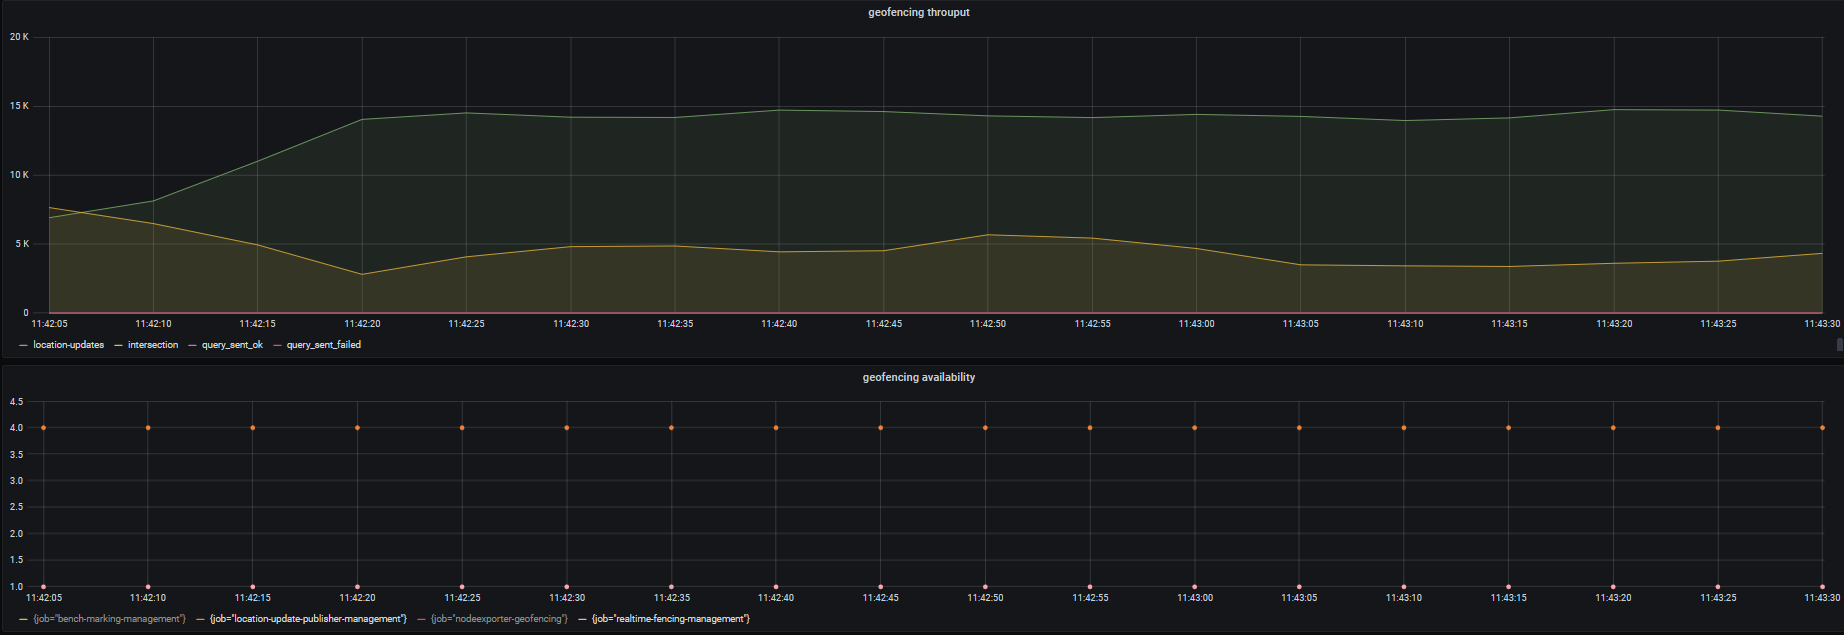
\includegraphics[scale=0.4]{images/evaluation/ex8-benchmarking-ongoing-2per4sec.png}
    \end{figure}

    In figure \ref{fig:ex8} the green line is essentially the input rate (number of location updates per second),
    yellow line represents throughput (number of fence point intersections) and the pink dots shows number of
    deployed instances of realtime-fencing.
    Figures in following push leg strong scalability experiments can also be read in the same way as experiment 8.

    So \ref{fig:ex8} illustrates that one instance of realtime-fencing with the rather low given resources, can only
    handle one 3rd (5K out of 15K) of input rate.

    \subsubsection{Experiment 9}

    \paragraph{Deployment view}
    \begin{center}
        \begin{tabular}{ c c c c }
            Application               & number of instances & CPU(MHz) & RAM(MB) \\
            location-update-publisher & 4                   & 200      & 700     \\
            location-aggregate        & 0                   & 2700     & 2700    \\
            realtime-fencing          & 2                   & 30       & 500     \\
        \end{tabular}
    \end{center}

    \paragraph{Result}
    \begin{figure}[ht]
        \caption{FenceX push leg strong scalability ex9}
        \label{fig:ex9}
        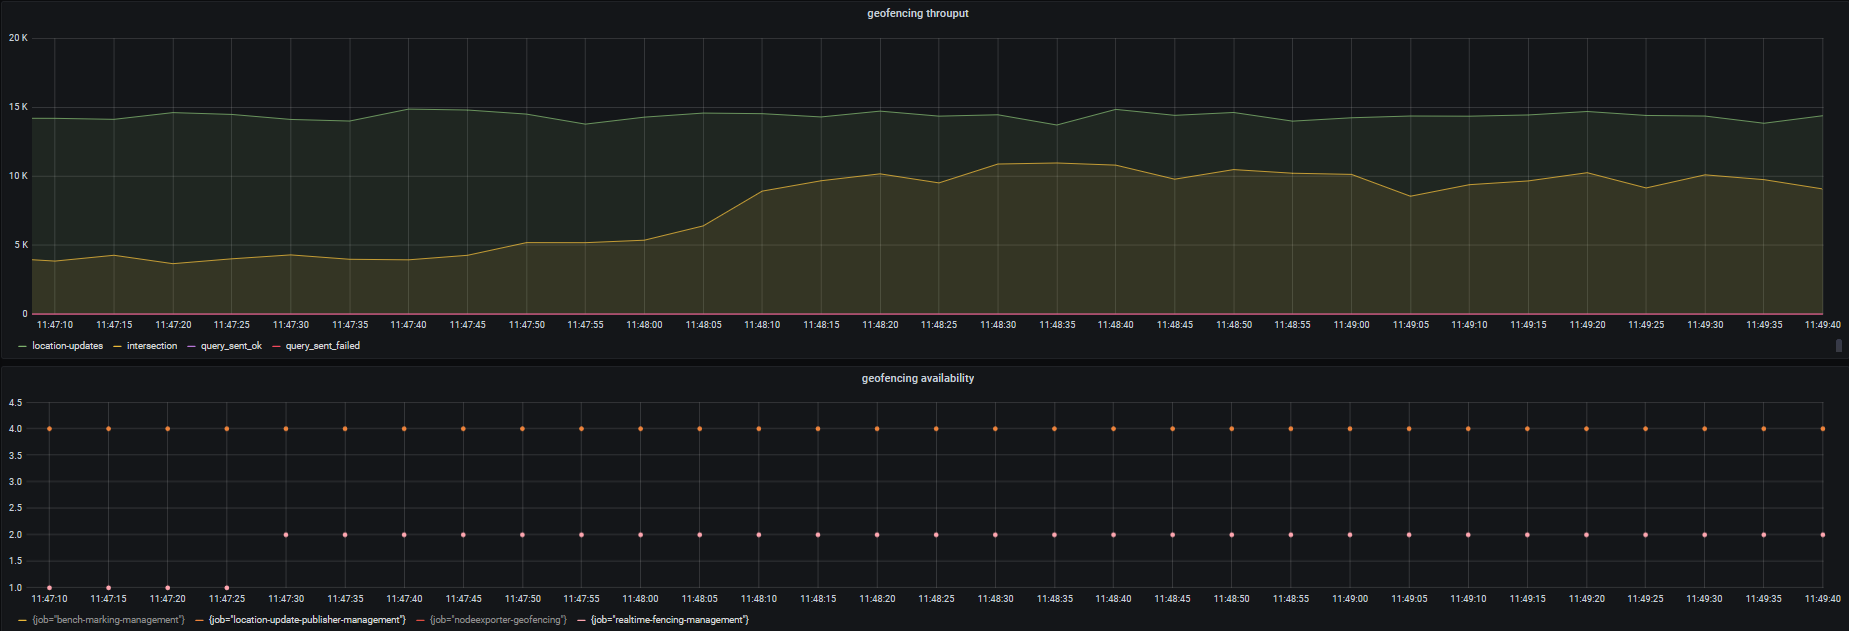
\includegraphics[scale=0.4]{images/evaluation/ex9-benchmarking-ongoing-2per4sec.png}
    \end{figure}

    Looking at figure \ref{fig:ex9} we can easily observ that once the second instance is up and running, after
    re-balancing, throughput goes proportionally up.
    From 5k/s to 10k/s.
    At this point we can guess that without chaning anything, just adding one more instance of realtime-fencing
    should be enough to cover the whole 15k/s input rate.
    15K location updates per second is the highest input rate that we could produce in a stable manner.

    \subsubsection{Experiment 10}

    \paragraph{Deployment view}
    \begin{center}
        \begin{tabular}{ c c c c }
            Application               & number of instances & CPU(MHz) & RAM(MB) \\
            location-update-publisher & 4                   & 200      & 700     \\
            location-aggregate        & 0                   & 2700     & 2700    \\
            realtime-fencing          & 3                   & 30       & 500     \\
        \end{tabular}
    \end{center}

    \paragraph{Result}
    \begin{figure}[ht]
        \caption{FenceX push leg strong scalability ex10}
        \label{fig:ex10}
        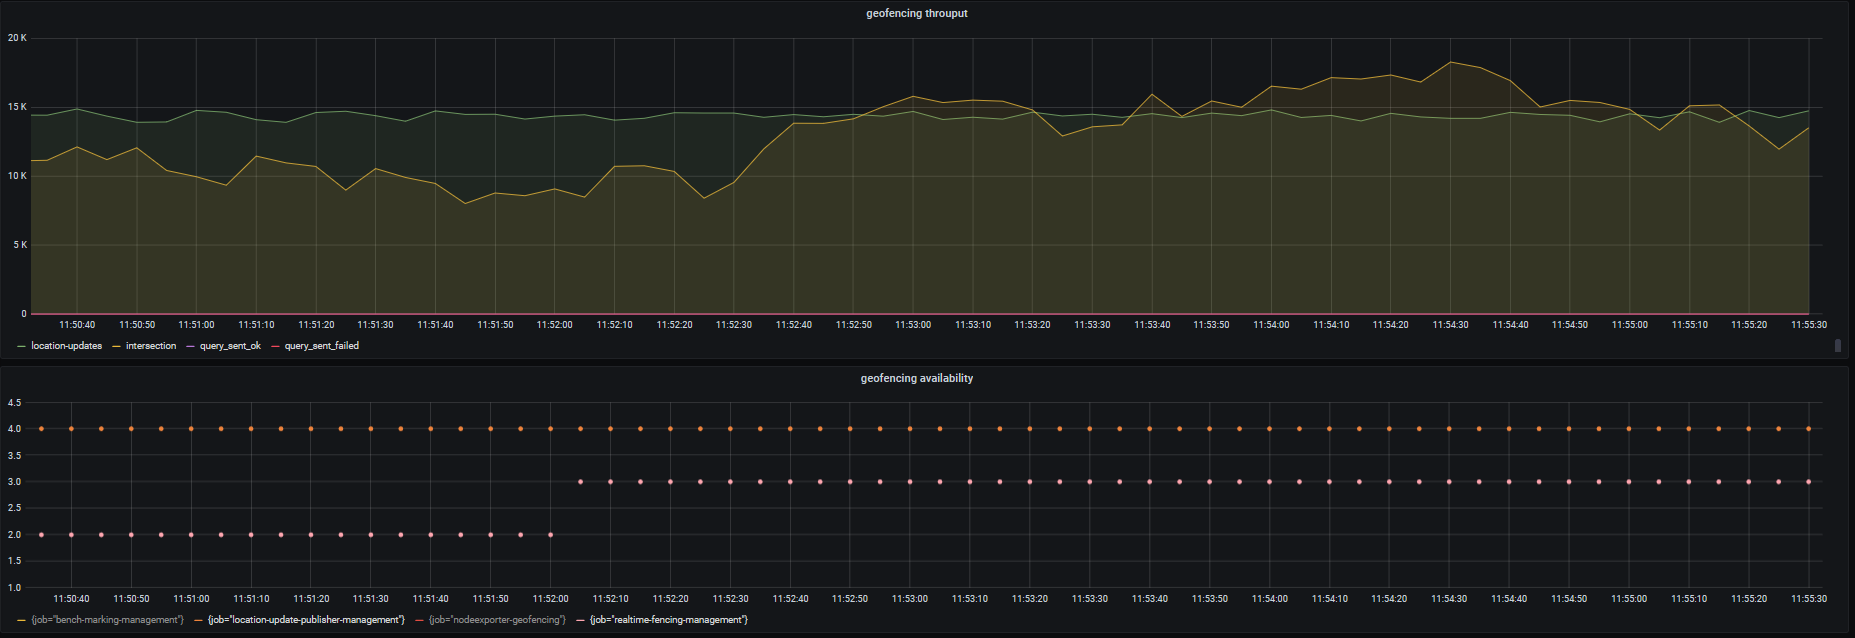
\includegraphics[scale=0.4]{images/evaluation/ex10-benchmarking-ongoing-2per4sec.png}
    \end{figure}
    As we expected, deploying three instances of realtime-fencing with the given resources, was enough to process 15K
    location updates per second.
    Also in \ref{fig:ex10} we can see effect of buffered location updates on throughput.
    Around the end parts of the graph, throughput is higher than input rate.

    \subsubsection{Experiment 11}
    Now in order to be just sure that adding more instances, won't affect the throughput in any good or bad way, we
    add another instance as the final step.

    \paragraph{Deployment view}
    \begin{center}
        \begin{tabular}{ c c c c }
            Application               & number of instances & CPU(MHz) & RAM(MB) \\
            location-update-publisher & 4                   & 200      & 700     \\
            location-aggregate        & 0                   & 2700     & 2700    \\
            realtime-fencing          & 4                   & 30       & 500     \\
        \end{tabular}
    \end{center}

    \paragraph{Result}
    \begin{figure}[ht]
        \caption{FenceX push leg strong scalability ex11}
        \label{fig:ex11}
        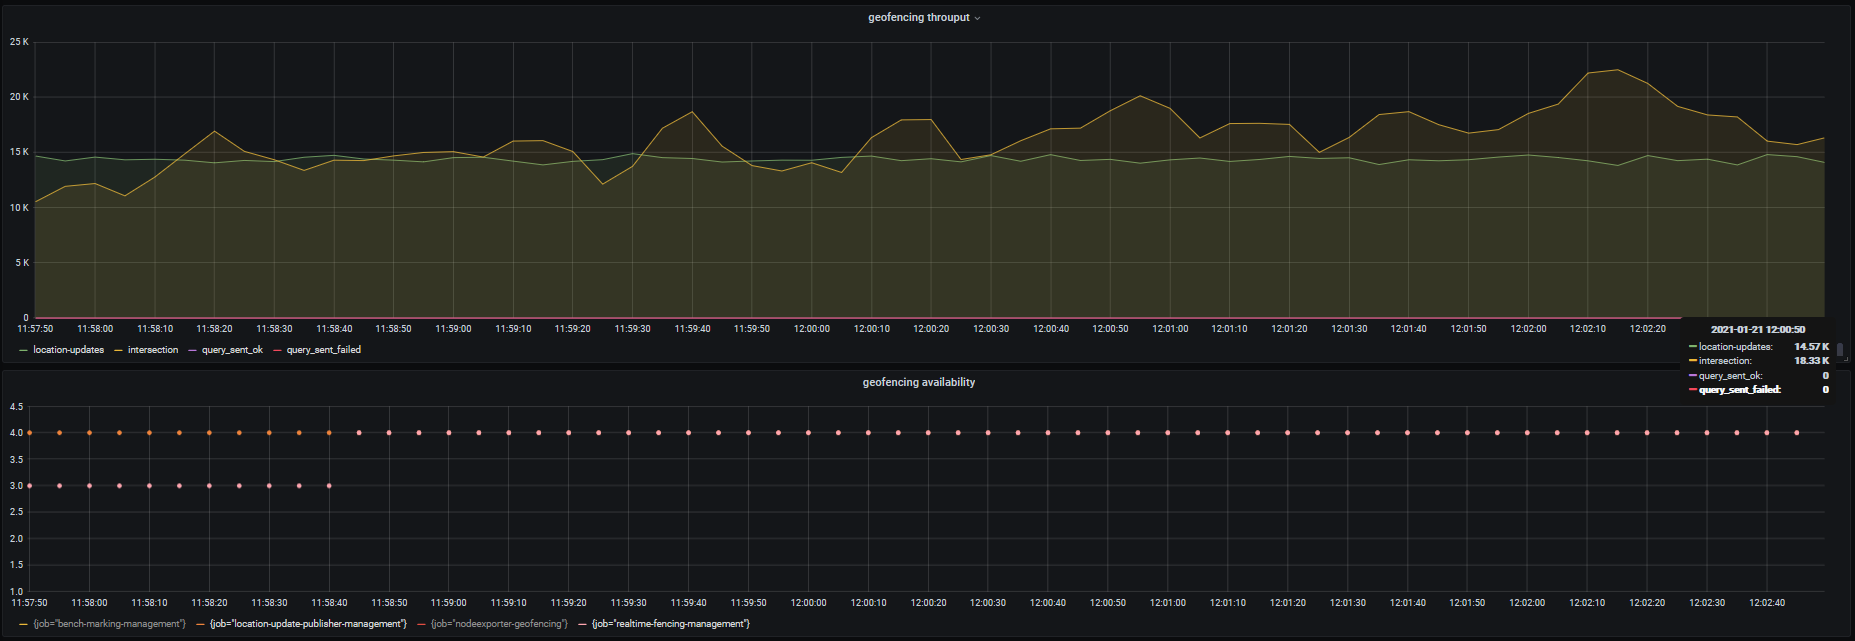
\includegraphics[scale=0.4]{images/evaluation/ex11-benchmarking-ongoing-2per4sec.png}
    \end{figure}
    The clear observation is that adding one more instance didn't have any special effect on the throughput.
    This is expected since throughput can not exceed input rate regardless of processing power.
    However, we can again see the effect of buffered location updates during re-balancing pretty much all over the
    graph.

    \subsection{Poll leg}
    The process of poll leg strong scalability experiments are as following:
    \begin{itemize}
        \item[1-] Send location reports for movers using all the trips in the bench-marking application database.
        \item[2-] Start an ongoing load of queries (query by fence) with fixed rate.
        \item[3-] Deploy only one instance of location-aggregate (should not be too rich in resources, we want it to be
        overwhelmed).
        \item[4-] Check the throughput. Hopefully it is much lower than the input rate.
        \item[5-] Deploy one more instances of location-aggregate with exactly same resources as previous one.
        \item[6-] Assert an increase in throughput.
        \item[7-] Keep adding instances and asserting increase in throughput until throughput stops increasing.
    \end{itemize}

    During these experiments, each time we deploy one more instance of location-aggregate, a re-balancing happens which
    avoids some queries from being answered.
    Those queries will be considered as failed.

    \subsubsection{Experiment 17}

    \paragraph{Deployment view}
    \begin{center}
        \begin{tabular}{ c c c c }
            Application               & number of instances & CPU(MHz) & RAM(MB) \\
            location-update-publisher & 0                   & 200      & 700     \\
            location-aggregate        & 1                   & 100      & 1500    \\
            realtime-fencing          & 0                   & 30       & 500     \\
        \end{tabular}
    \end{center}

    \paragraph{Result}
    \begin{figure}[ht]
        \caption{FenceX poll leg strong scalability ex17}
        \label{fig:ex17}
        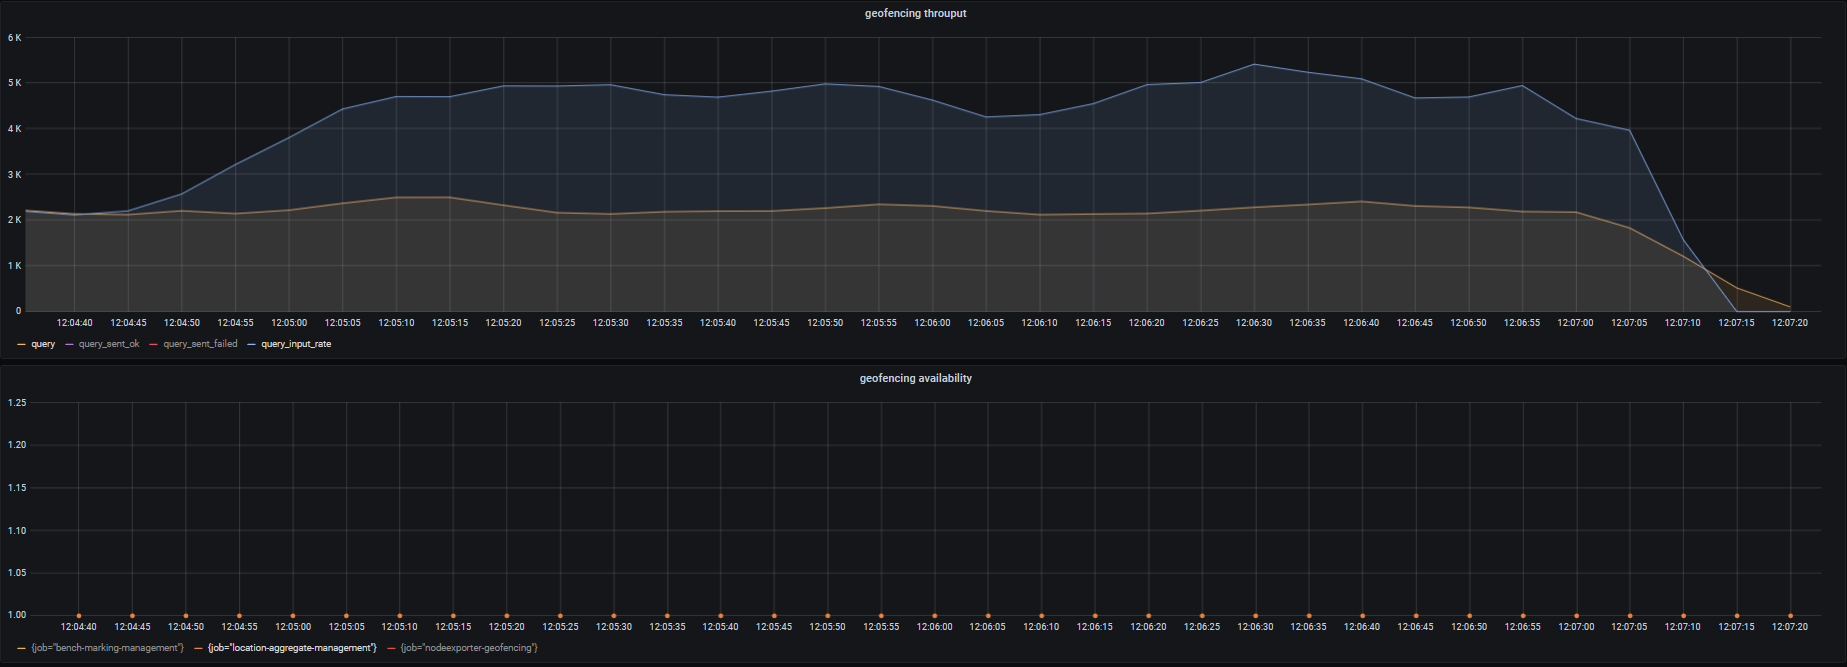
\includegraphics[scale=0.4]{images/evaluation/ex17-benchmarking-ongoing-2per4sec.png}
    \end{figure}

    \subsubsection{Experiment 18}

    \paragraph{Deployment view}
    \begin{center}
        \begin{tabular}{ c c c c }
            Application               & number of instances & CPU(MHz) & RAM(MB) \\
            location-update-publisher & 0                   & 200      & 700     \\
            location-aggregate        & 2                   & 100      & 1500    \\
            realtime-fencing          & 0                   & 30       & 500     \\
        \end{tabular}
    \end{center}

    \paragraph{Result}
    \begin{figure}[ht]
        \caption{FenceX poll leg strong scalability ex18}
        \label{fig:ex18}
        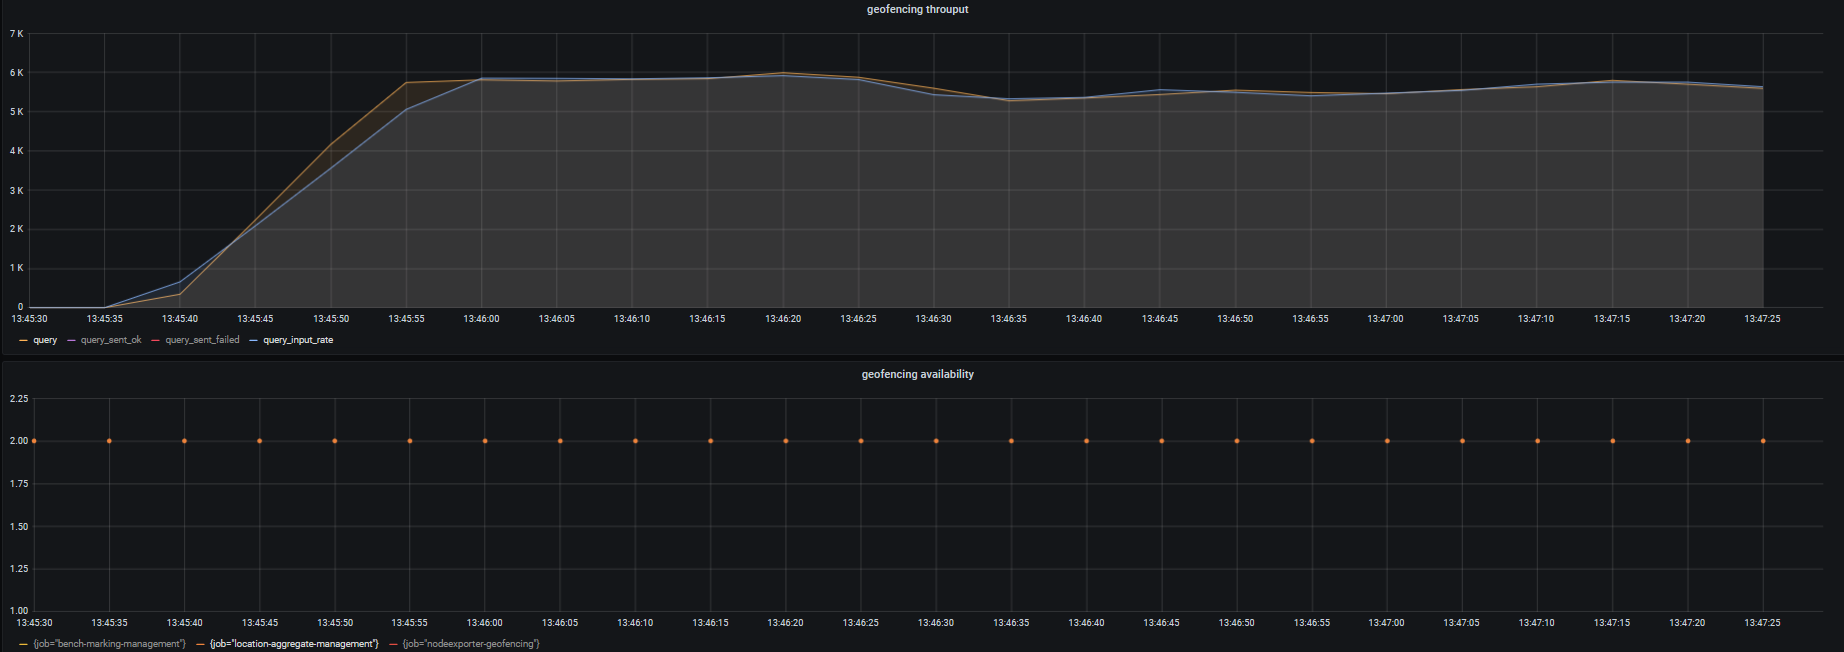
\includegraphics[scale=0.4]{images/evaluation/ex18-benchmarking-ongoing-2per4sec.png}
    \end{figure}

    In figures \ref{fig:ex17} and \ref{fig:ex18} the blue line is represents input rate, number of incoming HTTP
    requests.
    Orange line illustrates throughput which is number of queries responded successully.
    Orange dots also, show how many instances of location-aggregate are up and running.
    As figures show, FenceX has managed to handle 2k queries
    per second with one not so much rich instance of location-aggregate.
    Adding one more instance resulted in throughput becoming equal to input rate (~6K queries per second).

    One of the differences between push and poll leg is that, minimum resources required for poll leg to function
    smoothly is much higher than push leg.
    This is due to the fact that poll leg has global in memory data store.
    Also, the amount of data exists in poll leg is substantially higher.
    There is usually way more location updates for each mover than fences.
    In fact currently, there will be at most one fence in push leg for each mover compared to many location updates
    in poll leg.
    Please note that at each instance in time, there is only one location record for each mover in location-agreggate
    database (not many).
    But it processes more than one location update for each mover over time.

    As an overall consequence, when we deploy even one instance of location-aggregate, it's already rich enough to be
    able to answer many HTTP requests (query by fence).
    About half of the input rate we can produce at maximum in a stable ongoing manner.
    So there is no point in continuing strong scalability experiments for poll leg withing this range of input.


    \section{Weak scalability}
    If a software has weak scalability properties, it means providing a load which is increasing step by step over
    time, the more you scale the software out, the better it performs.
    For a given circumstance, there might be a point after which more scale out or more load won't affect
    the performance anymore.
    The load can be data set size, table size, incoming http query rate and ... .
    Performance is also case and context dependent.
    It can be query latency, throughput and ... .
    In stream processing systems, load is the rate of input, rate of incoming events, the rate at
    which source publishes input in to the piple line.
    In FenceX, for poll leg, similar to previous experiments, load is rate of incoming HTTP requests for queries by
    fence.
    And, for push leg is the rate at which location reports arrive.

    Performance in case of our experiments for FenceX specifically, is throughput of push leg and poll leg.

    \subsection{Push leg}
    The process of weak scalability experiments are as following:
    \begin{itemize}
        \item[1-] Define fences for movers using all the trips in the bench-marking application database.
        \item[2-] Start an ongoing stream of location report with fixed low rate toward FenceX.
        \item[3-] Deploy only one instance of realtime-fencing (should not be too rich in resources, we want it to
        be overwhelmed).
        \item[4-] Check the throughput. Hopefully it is equal to input rate.
        \item[5-] Deploy one more instances of realtime-fencing with exactly same resources as previous one. Also,
        increase the input rate (like double).
        \item[6-] Assert that throughput covers the input rate.
        \item[7-] Keep adding instances, increasing input rate and asserting increase in throughput until throughput
        stops increasing.
    \end{itemize}

    During these experiments, each time we deploy one more instance of realtime-fencing, a re-balancing happens which
    avoids some incoming location updates from being processed.
    Those location updates get buffered in the topic and after re-balancing will get their chance to be processed.
    A direct consequence of such buffering is that at some points in the experiments, the throughput we observe might be
    higher than the input rate.
    This is because the input stream is ongoing and fixed rate.

    \subsubsection{Experiment 19}

    \paragraph{Deployment view}
    \begin{center}
        \begin{tabular}{ c c c c }
            Application               & number of instances & CPU(MHz) & RAM(MB) \\
            location-update-publisher & 4                   & 400      & 700     \\
            location-aggregate        & 0                   & 2700     & 2700    \\
            realtime-fencing          & 1                   & 60       & 500     \\
        \end{tabular}
    \end{center}

    \paragraph{Result}
    \begin{figure}[ht]
        \caption{FenceX push leg weak scalability ex19}
        \label{fig:ex19}
        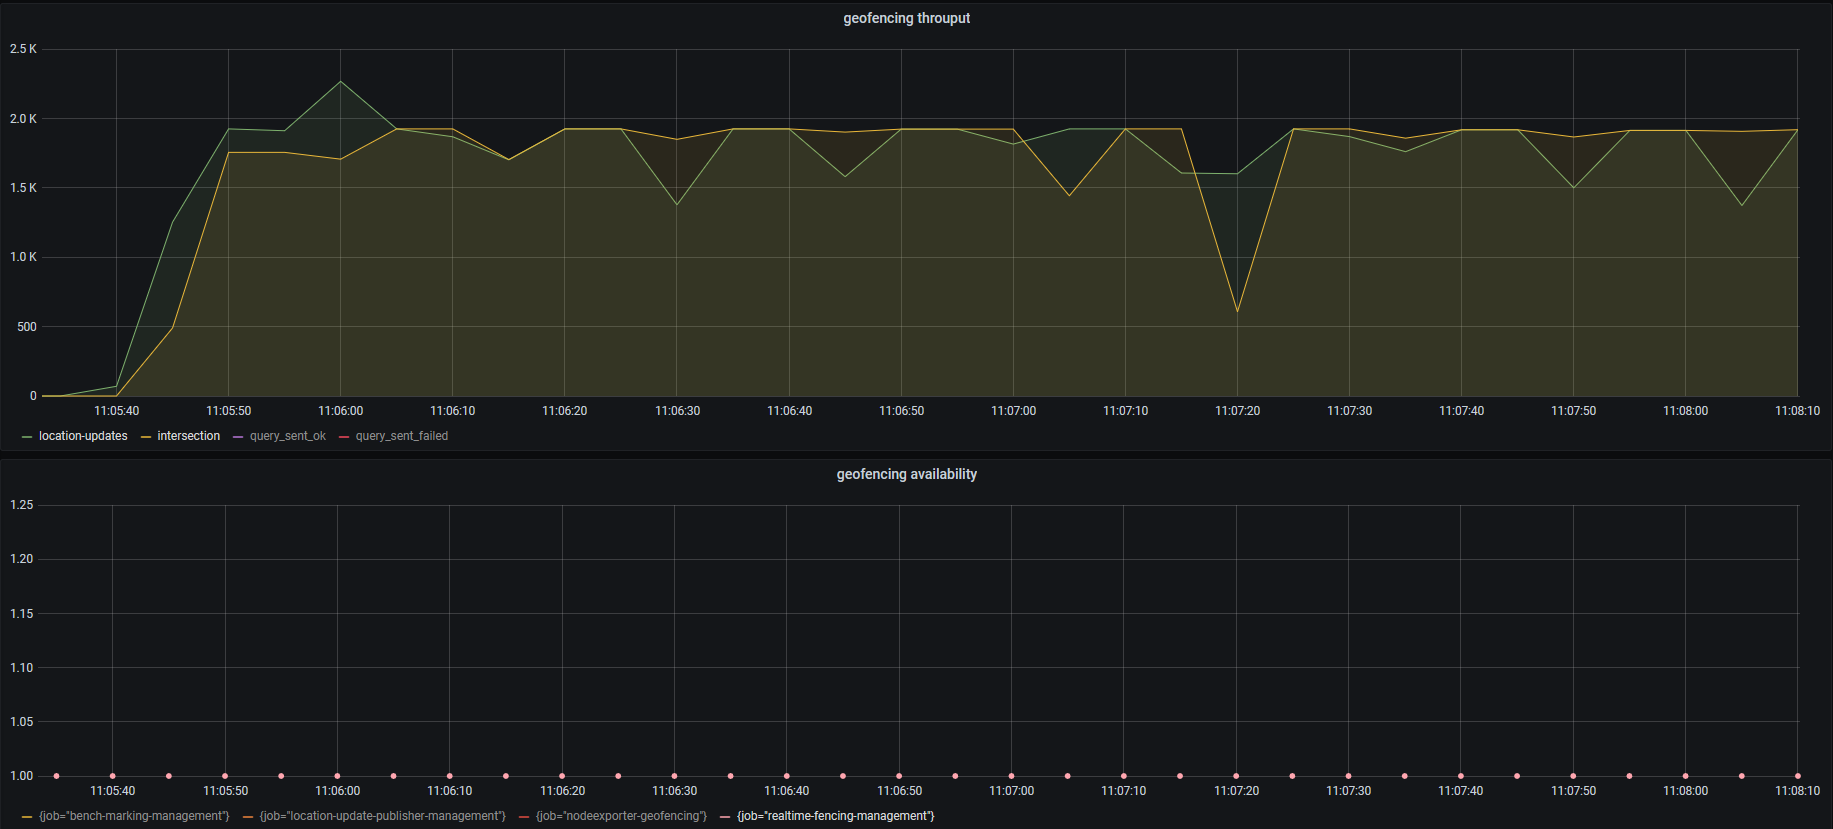
\includegraphics[scale=0.4]{images/evaluation/ex19-benchmarking-ongoing-1per16sec.png}
    \end{figure}

    In figure \ref{fig:ex19} the green line is input rate (number of location updates per second),
    yellow line represents throughput (number of fence point intersections) and the pink dots shows number of
    deployed instances of realtime-fencing.
    Figures in following push leg weak scalability experiments can also be read in the same way as experiment 19.

    So far with one limited in resources instance of realtime-fencing, FenceX has managed to deal with around 2K
    location updates per second succesfully in a stable manner.

    \subsubsection{Experiment 20}

    \paragraph{Deployment view}
    \begin{center}
        \begin{tabular}{ c c c c }
            Application               & number of instances & CPU(MHz) & RAM(MB) \\
            location-update-publisher & 4                   & 400      & 700     \\
            location-aggregate        & 0                   & 2700     & 2700    \\
            realtime-fencing          & 2                   & 60       & 500     \\
        \end{tabular}
    \end{center}

    \paragraph{Result}
    \begin{figure}[ht]
        \caption{FenceX push leg weak scalability ex20}
        \label{fig:ex20}
        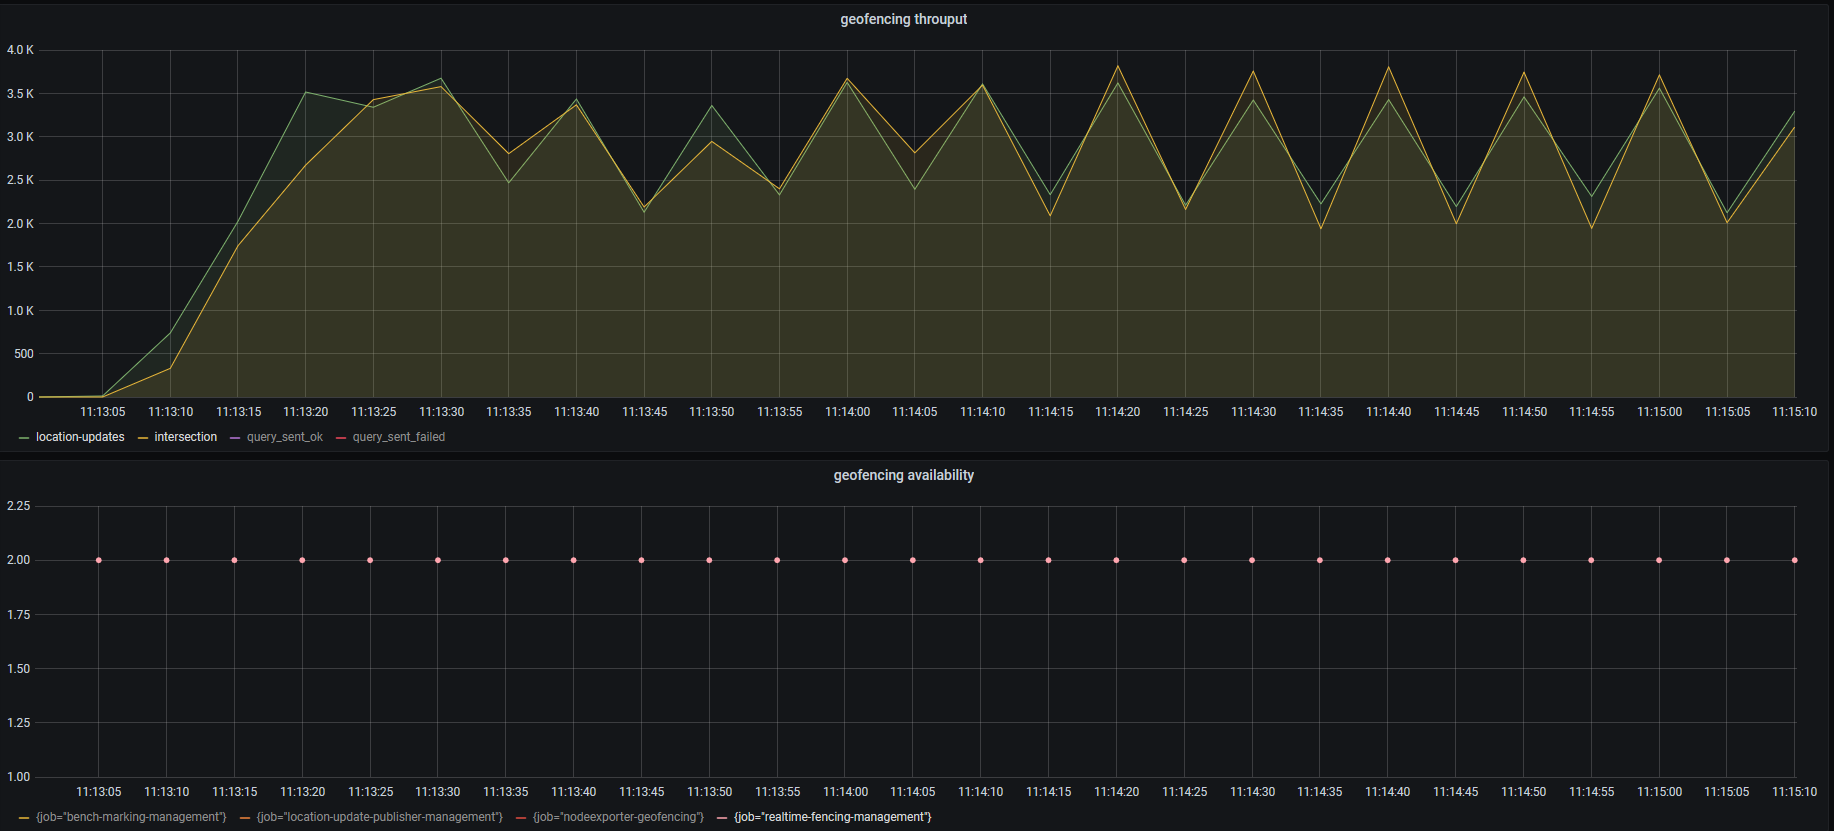
\includegraphics[scale=0.4]{images/evaluation/ex20-benchmarking-ongoing-1per10sec.png}
    \end{figure}

    Two such instances of realtime-fencing managed to handle around 3K location updates per second.

    \subsubsection{Experiment 21}

    \paragraph{Deployment view}
    \begin{center}
        \begin{tabular}{ c c c c }
            Application               & number of instances & CPU(MHz) & RAM(MB) \\
            location-update-publisher & 4                   & 400      & 700     \\
            location-aggregate        & 0                   & 2700     & 2700    \\
            realtime-fencing          & 4                   & 60       & 500     \\
        \end{tabular}
    \end{center}

    \paragraph{Result}
    \begin{figure}[ht]
        \caption{FenceX push leg weak scalability ex21}
        \label{fig:ex21}
        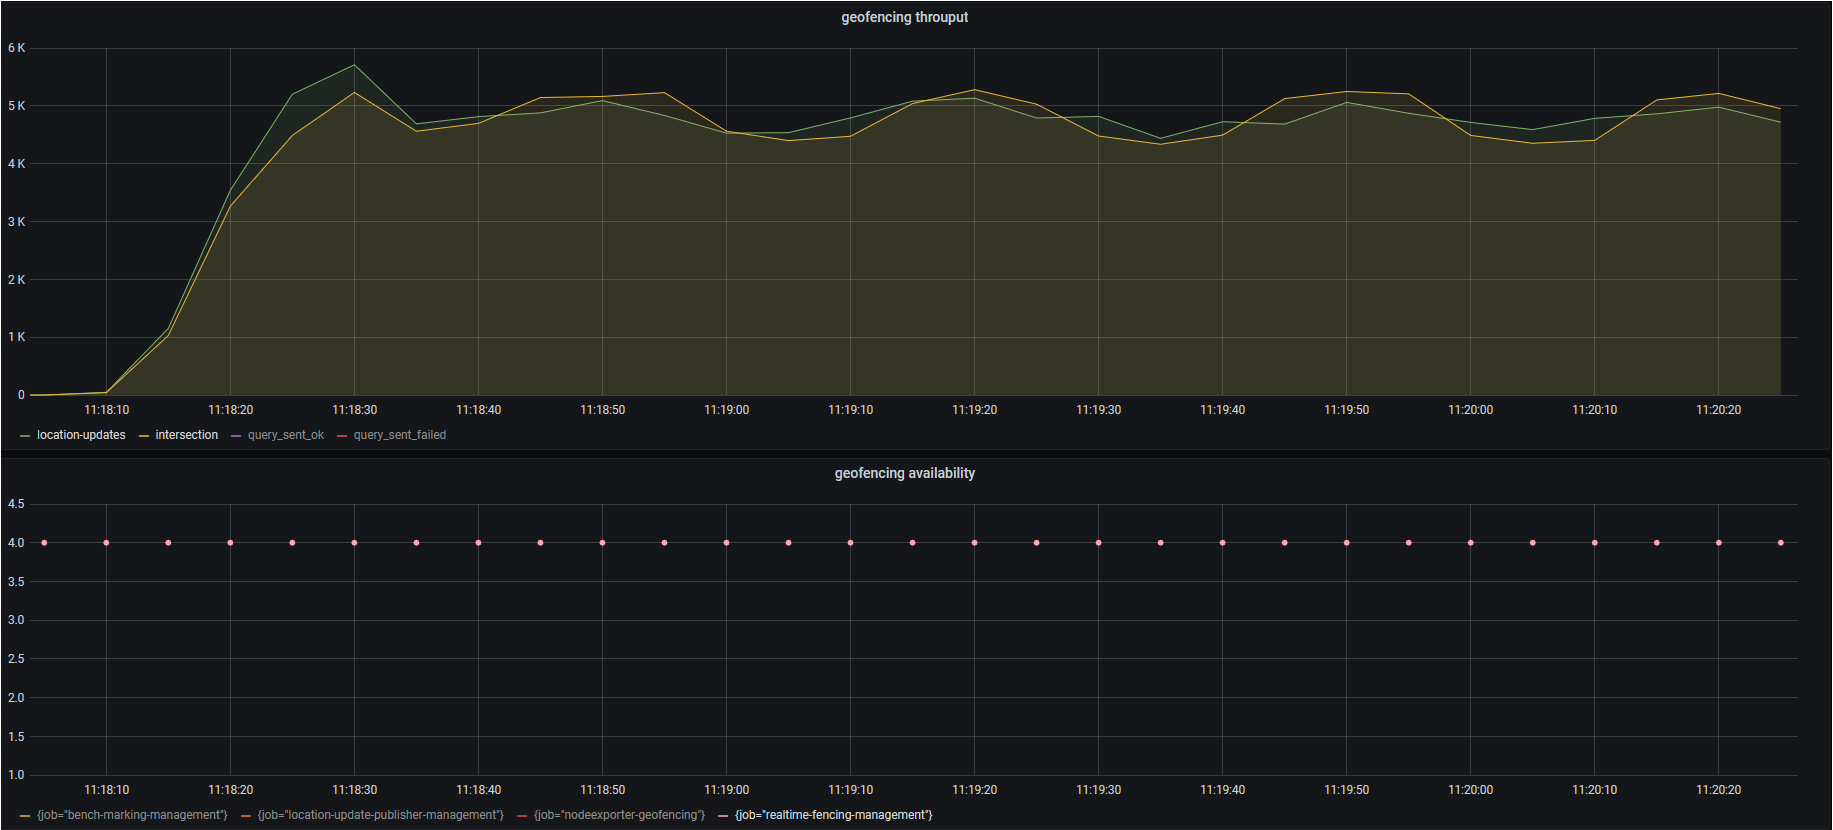
\includegraphics[scale=0.4]{images/evaluation/ex21-benchmarking-ongoing-1per6sec.png}
    \end{figure}
    Four such instances of realtime-fencing managed to handle around 5K location updates per second.

    \subsubsection{Experiment 22}

    \paragraph{Deployment view}
    \begin{center}
        \begin{tabular}{ c c c c }
            Application               & number of instances & CPU(MHz) & RAM(MB) \\
            location-update-publisher & 4                   & 400      & 700     \\
            location-aggregate        & 0                   & 2700     & 2700    \\
            realtime-fencing          & 5                   & 60       & 500     \\
        \end{tabular}
    \end{center}

    \paragraph{Result}
    \begin{figure}[ht]
        \caption{FenceX push leg weak scalability ex22}
        \label{fig:ex22}
        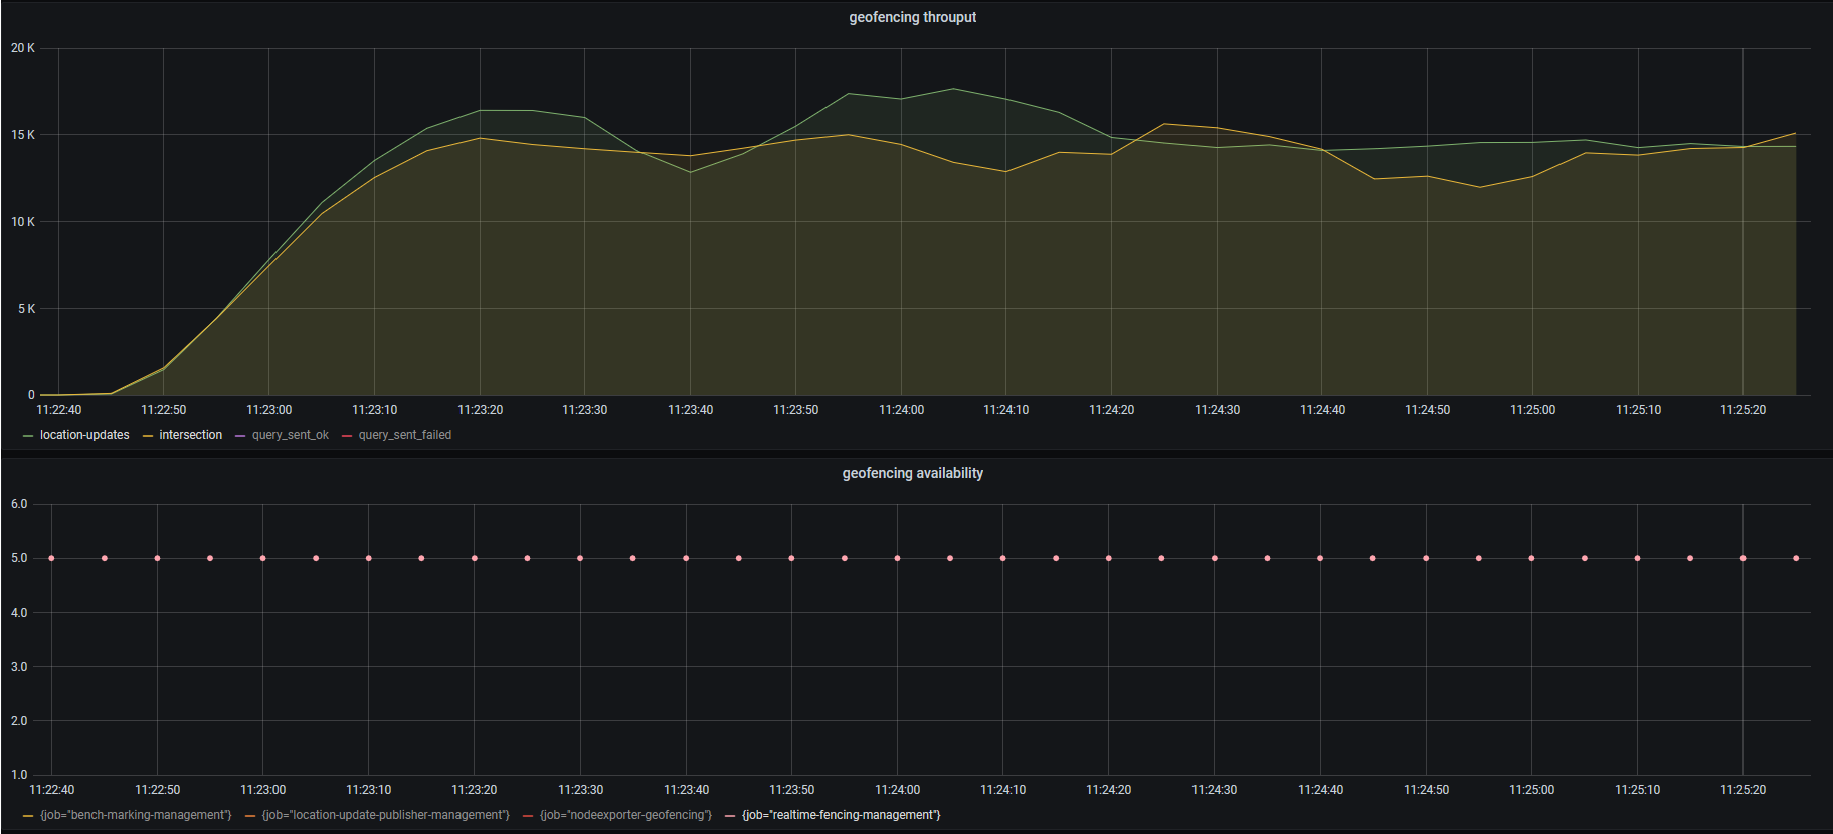
\includegraphics[scale=0.4]{images/evaluation/ex22-benchmarking-ongoing-1per2sec.png}
    \end{figure}
    Five such instances of realtime-fencing managed to handle around 15K location updates per second.

    \subsubsection{Experiment 23}

    \paragraph{Deployment view}
    \begin{center}
        \begin{tabular}{ c c c c }
            Application               & number of instances & CPU(MHz) & RAM(MB) \\
            location-update-publisher & 4                   & 400      & 700     \\
            location-aggregate        & 0                   & 2700     & 2700    \\
            realtime-fencing          & 10                  & 60       & 500     \\
        \end{tabular}
    \end{center}

    \paragraph{Result}
    \begin{figure}[ht]
        \caption{FenceX push leg weak scalability ex23}
        \label{fig:ex23}
        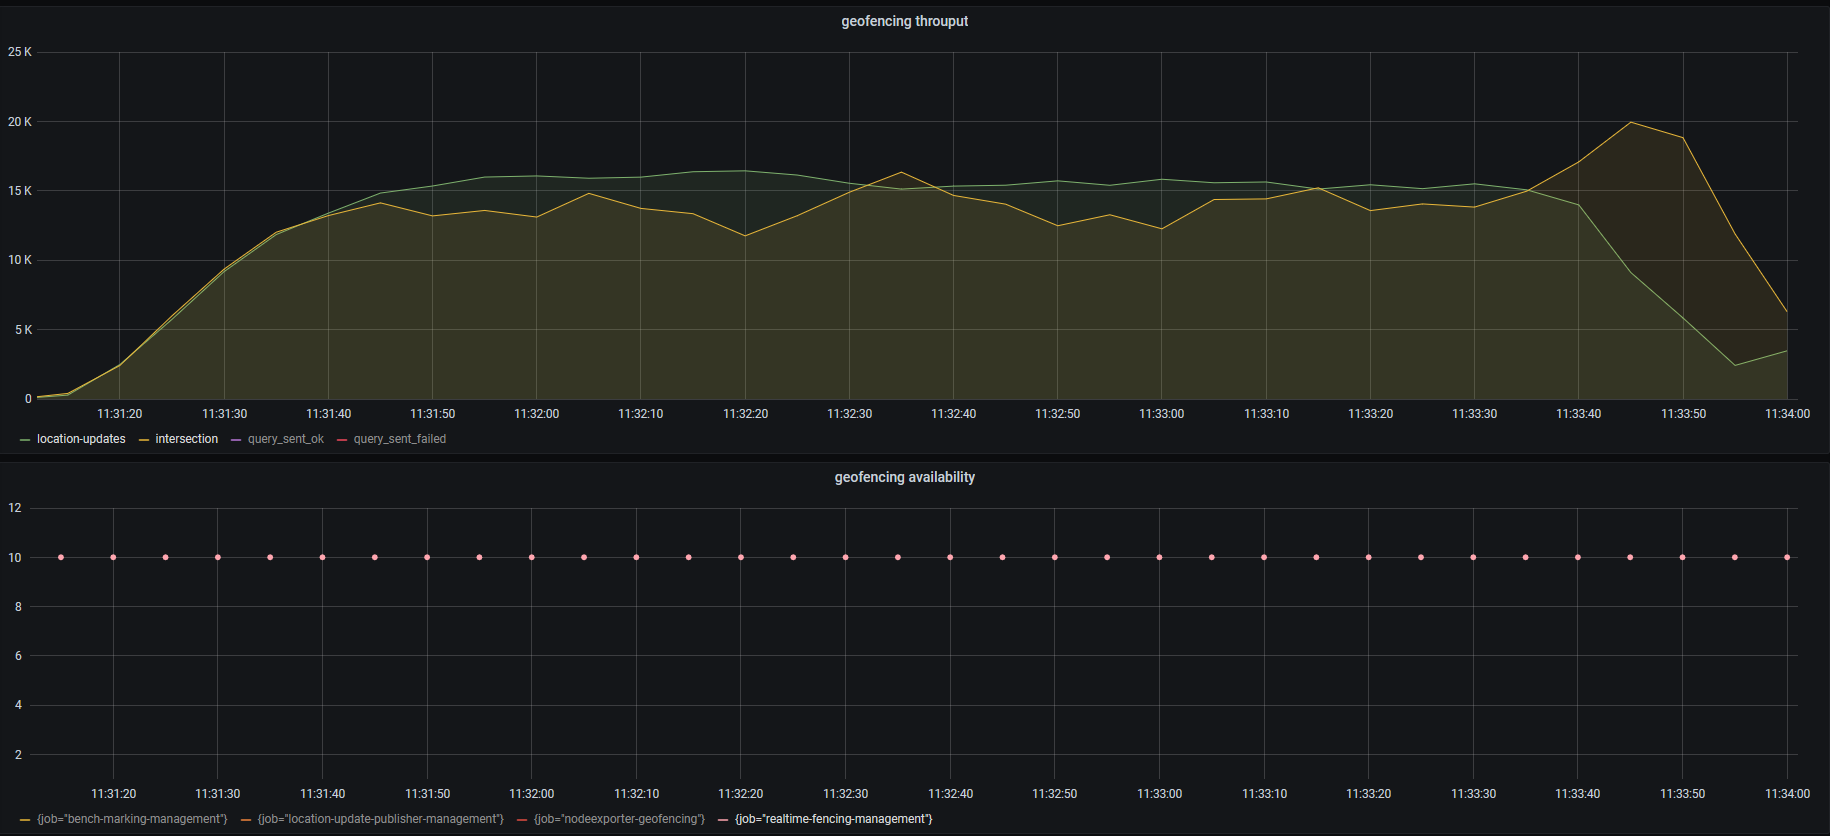
\includegraphics[scale=0.4]{images/evaluation/ex23-benchmarking-ongoing-2per2sec.png}
    \end{figure}
    Ten such instances of realtime-fencing managed to handle around 15K location updates per second.
    However, in experiment 23 our intention was to increase input rate to above 15k/s which we did not manage due to
    limitations on the available resources to bench-marking application.
    So we will not continue weak scalability experiments for push log further.
    We have concluded that push leg of FenceX managed to scale well in face of increasing load.

    \subsection{Poll leg}
    The process of poll leg weak scalability experiments are as following:
    \begin{itemize}
        \item[1-] Send location updates for movers using all the trips in the bench-marking application database.
        \item[2-] Start an ongoing load of queries (query by fence) with fixed low rate.
        \item[3-] Deploy only one instance of location-aggregate (should not be too rich in resources, we want it to
        be overwhelmed).
        \item[4-] Check the throughput. Hopefully it is equal to input rate.
        \item[5-] Deploy one more instances of location-aggregate with exactly same resources as previous one. Also,
        increase the input rate (like double).
        \item[6-] Assert that throughput covers the input rate.
        \item[7-] Keep adding instances, increasing input rate and asserting increase in throughput until throughput
        stops increasing.
    \end{itemize}

    Relaying on the observations from previous experiments, two instances of location-aggregate (with minimum
    resources for working smoothly) can easily cover our maximum capacity for producing input load.
    So there is no point in carrying out weak scalability experiments for poll leg.


    \section{Free fall scalability}
    In order to stress test stream processing systems or when trying to find out how they can scale under high rates
    of input load, naturally we need to be able to produce high rates of input in the first place.
    This can be challenging when the input data is complex to produce and/or available resources to our input
    producers is limited.
    Stream processing systems relay on some sort of buffering which means events should be stored somewhere so
    that processors can handle them when they are ready.
    That's how they get some sort of back pressure in reactive systems terminology.
    In case of FenceX, that buffer is the Kafka topics which can grow very large without any problem.

    So instead of trying to produce a high rate of input in realtime, we can buffer large number of events in a Kafka
    topic (waiting to be picked up and processed) while processors are down.
    When enough events got accumulated, we stop buffering event and deploy event processors.
    Now processors can read the events with the least possible IO involved.
    Applying this approach, we can assess how well an event processor can be scaled when there is almost no factor
    involved other than input rate and processing power.

    This style of testing is only applicable to push leg since the concept of buffering work differently in terms of
    HTTP request.
    Basically HTTP based communication does not support back pressure.

    \subsection{Push leg}
    The process of free fall scalability experiment is as following:
    \begin{itemize}
        \item[1-] Play with different input rates and deployment configurations to get a feeling of how to tune the
        system for best performance
        \item[2-] Undeploy all realtime-fencing instances.
        \item[3-] Start an ongoing stream of location report with fixed rate toward FenceX.
        \item[4-] Wait 5 minutes or so.
        \item[5-] Now that there is plenty of location updates buffered in the Kafka topic, stop the stream of
        location updates.
        \item[6-] Deploy realtime-fencing instances according to the previously discovered deployment configuration.
        \item[7-] Check the throughput and assert that it's much higher than maxixmum oberserved throughput in
        previous experiments.
    \end{itemize}

    \subsubsection{Experiment 24}

    \paragraph{Deployment view}
    \begin{center}
        \begin{tabular}{ c c c c }
            Application               & number of instances & CPU(MHz) & RAM(MB) \\
            location-update-publisher & 4 - 0               & 400      & 700     \\
            location-aggregate        & 0                   & 2700     & 2700    \\
            realtime-fencing          & 0 - 12              & 60       & 500     \\
        \end{tabular}
    \end{center}

    \paragraph{Result}
    \begin{figure}[ht]
        \caption{FenceX push leg free fall scalability ex24}
        \label{fig:ex24}
        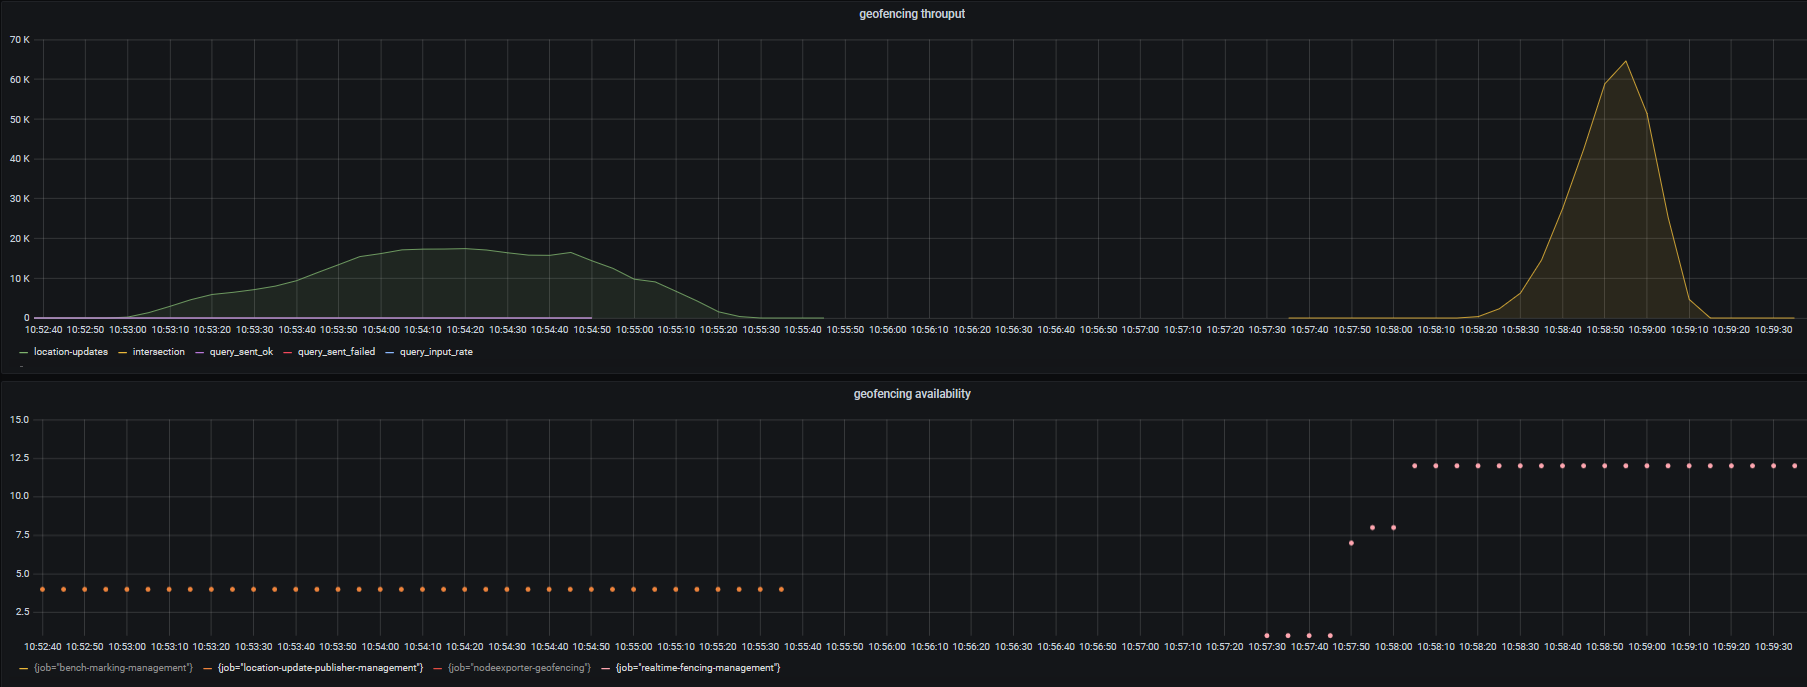
\includegraphics[scale=0.4]{images/evaluation/ex24-benchmarking-ongoing-1per2sec.png}
    \end{figure}
    In figure \ref{fig:ex24} the green line is input rate (number of location updates per second),
    yellow line represents throughput (number of fence point intersections) and the pink dots shows number of
    deployed instances of realtime-fencing.
    Orange dots illustrates number of up and running instances of location-update-publisher.
    We can clearly observe that after re-balancing among 10 newly deployed instance of realtime-fencing is finished,
    throughput has picked very fast to about 65K fence-point intersections per second.

    \section{Related work}
    In this section we will go over two papers which has introduced geofencing systems.

    \subsection{Large Scale Indexing of Geofences}
    In this article, a poll style on demand geofencing system is introduced that supports large scales
    of data and load.
    This system has a concept of worker which refers to instances of application that answer to queries.
    As apposed to clients which send queries to the worker nodes.
    Dynamic caching and work load distribution over multiple instances of workers are the bases of achieved
    scalability.

    Each worker instance is responsible for indexing a region of the world, which allows for lower query and index latency.
    Since each worker instance is responsible for different part of the world, queries targeting border areas need
    special treatment.
    As a solution, each worker instance also is responsible for areas around its dedicated region.

    It is notable that software in \cite{Cirillo_Jacobs_Martin_Szczytowski_2014} uses a custom geospatial index,
    custom design and implementation.
    Using a custom index most probably means that the whole data is stored and processed in memory which allows for higher throughput.
    We will not, however, describe further the indexing strategy since it is outside context of this thesis.

    Throughput in \cite{Cirillo_Jacobs_Martin_Szczytowski_2014} is defined as number of location updates processed per second.
    Such processing involves updating an index plus a query to find a crossing geofence.

    When they are using benefit of localhost communication without any data replication involved (no availability), a
    throughput of 250k/s has been achieved on average.
    However, once they introduce data replication and inter server communication, the throughout drops to sub 10k/s
    range at best.

    \subsubsection{Comparison}
    The software introduced in \cite{Cirillo_Jacobs_Martin_Szczytowski_2014}, although having notification
    functionalities, is comparable to poll leg of FenceX.
    Both of them use load sharing (scale out) and in-memory data processing to achieve high throughput and
    scalability.

    FenceX, however, does not apply partitioning data among worker instances in poll leg, which makes it much easier to
    scale out.
    Also, the load balancing strategy when forwarding client queries to worker instances can be as simple as
    round-robin in FenceX.
    As a result, no throughput would be lost during load balancing.

    When it comes to numbers, FenceX has acheived a throughput in range of 15k/s compared to sub 10k/s for
    \cite{Cirillo_Jacobs_Martin_Szczytowski_2014}.
    Although \cite{Cirillo_Jacobs_Martin_Szczytowski_2014} has done wonderful when no availability was in action
    (no replication), we do not consider it a win over FenceX.
    FenceX has always been tested with full replication in action.
    So all in all, FenceX has achieved a higher throughout.

    \subsection{Using Complex Event Processing for implementing a geofencing service}
    \cite{Târnaucă_Puiu_Nechifor_Comnac_2013} introduces a push style realtime geofencing system that relies on a CEP
    (complex event processing) for fence entrance/exit detection.
    Which is comparable to functionalities of push leg of FenceX when realtime fence point intersections happen.
    System in \cite{Târnaucă_Puiu_Nechifor_Comnac_2013} is using a classic 3 tiers monolith architecture.
    Unit of concurrency of in \cite{Târnaucă_Puiu_Nechifor_Comnac_2013} is not clear. So it's not clear what are the
    bounds for scalability of the introduced system.

    Throughput in this system is defined as number of location updates processed per second.
    Evaluations have shown that it can has achieved throughput of around 20k/s.

    \subsubsection{Comparison}
    Unlike FenceX, \cite{Târnaucă_Puiu_Nechifor_Comnac_2013} does not seem to have any considerations for
    scalability and availability.
    Also when it comes to throughput, push leg of FenceX has achieved 65k/s which is much higher than 20k/s.



    \nocite{*}
    \bibliography{sources}
    \bibliographystyle{IEEEtran}
\end{document}
